\documentclass[10pt, a4paper]{article}
\usepackage{lrec}
%\usepackage{multibib}
%\newcites{languageresource}{Language Resources}
\usepackage{graphicx}
\usepackage{tabularx}
\usepackage{soul}
% for eps graphics
\usepackage[usenames, dvipsnames]{color}

\usepackage{epstopdf}
\usepackage[latin1]{inputenc}
\usepackage{xspace}
\usepackage{booktabs}
\usepackage{hyperref}
\usepackage{xstring}
\usepackage{xspace}
\usepackage{multirow}
\usepackage{colortbl}
\usepackage{xcolor}

\usepackage{microtype}

\newcommand{\secref}[1]{\StrSubstitute{\getrefnumber{#1}}{.}{ }}

\newcommand{\refexp}[1]{\textsl{#1}}
\newcommand{\word}[1]{\textsl{#1}}
\newcommand{\cat}[1]{\textsc{#1}}
\newcommand{\domain}[1]{\textsc{#1}}
\newcommand{\vgenome}{VisualGenome\xspace}
\newcommand{\vg}{VG\xspace}
\newcommand{\ra}{$\rightarrow$}
\newcommand{\referit}{ReferIt\xspace}
\newcommand{\refcoco}{RefCOCO\xspace}
\newcommand{\refcocop}{RefCOCO+\xspace}
\newcommand{\flickr}{Flickr30k Entities\xspace}

\newcommand{\sz}[1]{\textcolor{blue}{\emph{//sz: #1//}}}
\newcommand{\gbt}[1]{\textcolor{orange}{\emph{//g: #1//}}}
\newcommand{\cs}[1]{\textcolor{green!60!black}{\emph{//cs: #1//}}}

\definecolor{lightgray}{gray}{0.85}

\title{Object Naming in Language and Vision: A Survey and a New Dataset}

\name{Carina Silberer, Sina Zarrie\ss, Gemma Boleda}

\address{Universitat Pompeu Fabra, University of Jena, Universitat Pompeu Fabra \\
         Barcelona (Spain), Jena (Germany), Barcelona (Spain) \\
         sina.zarriess@uni-jena.de\\
         \{carina.silberer, gemma.boleda\}@upf.edu\\}


\abstract{
People choose particular names for objects, such as \word{dog} or \word{puppy} for a given dog.
Object naming has been studied in Psycholinguistics, but has received relatively little attention in Computational Linguistics.
We review resources from Language and Vision that could be used to study object naming on a large scale, discuss their shortcomings, and create a new dataset that affords more opportunities for analysis and modeling.
Our dataset, ManyNames, provides 36 name annotations for each of 25K objects in images selected from VisualGenome.
We highlight the challenges involved and provide a preliminary analysis of the ManyNames data showing that there is a high level of agreement in naming, on average. At the same time, the average number of name types associated with an object is much higher in our dataset than in existing corpora for Language and Vision, such that ManyNames provides a rich resource for studying phenomena like taxonomic variation (\word{chihuahua} vs.\ \word{dog}), which has been discussed a lot in the theoretical literature, and other less well studied phenomena like cross-classification (\word{cake} vs.\ \word{dessert}).
% may not be the main driver of diversity in naming behavior, \cs{sounds weird:}at least in our setup.\cs{in naming behavior on real-world objects (?)}
 \\ \newline \Keywords{object naming, language and vision, computer vision} }

\begin{document}

\maketitleabstract

\cs{maybe streamline use of (i),(ii),... and (1),(2),...}
\section{Introduction}
\begin{figure}[tbp]
\begin{tabular}{p{2.5cm}p{2.5cm}}
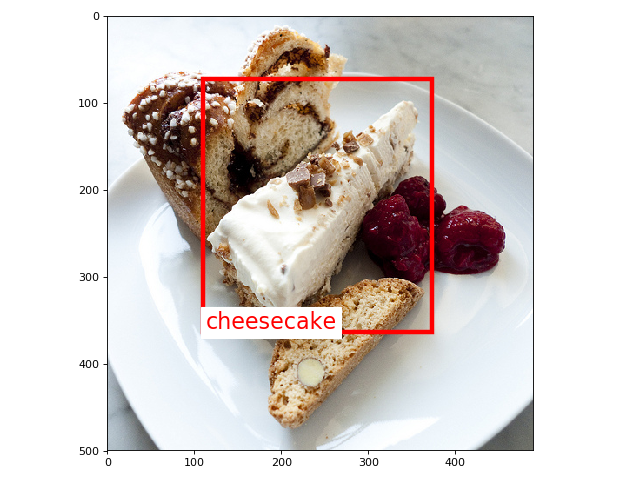
\includegraphics[height=3cm]{figures/cheesecake.png} &
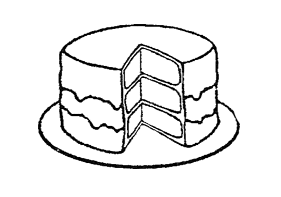
\includegraphics[height=3cm]{figures/snodgrass_vanderwart_cake_042.png}
\end{tabular}
\caption{Object name from VisualGenome. Names like \refexp{cake}, \refexp{dessert}, \refexp{sweet}, or \refexp{food} would be valid, too.}
\label{fig:cake}
\vspace{-0.5cm}
\end{figure}

Determining object names, such as \emph{cheesecake} for the marked object in Figure~\ref{fig:cake}, is a core aspect of virtually every language \& vision task, ranging from e.g.\ referring expression generation to visual dialogue \cite{fangetal:2015,devlin:imcaqui,Bernardietal:automatic,das2017visual,vries2017guesswhat}.
%While many of these tasks are well-known to 
%\gbt{I've left only one image in the figure to highlight that we study variation for the same instance.}
However, so far research in NLP has had surprisingly little to say about object naming.
Neighboring areas
%, specifically Computer Vision and Cognitive Science, 
have addressed related tasks, with simplifications that NLP is equipped to address:
In Computer Vision, naming is usually equated with object categorization, and addressed as a classification problem in which a single label is provided for each object~\cite{googlenet}.
%In a typical evaluation, alternative names for the object in Figure \ref{fig:cake} such as \refexp{cake}, \refexp{dessert}, \refexp{sweet}, or \refexp{food} would be counted as incorrect.
In Cognitive Science, object naming has received more attention, but it has been studied with stylized drawings instead of realistic images.
%, such that it is unclear how findings generalize to tasks in language \& vision.

We take a first step at studying naming of object in real-world images and contribute a new dataset, ManyNames, that contains 36 crowd-sourced names for 25K instances from VisualGenome~\cite{krishna2016visualgenome}.
Thus, our images show objects in complex visual contexts
%, surrounded by other objects, 
unlike the ``clean'' ImageNet data~\cite{imagenet_cvpr09} that has been previously used to train object or name classifiers \cite{Ordonez:2016}.

We find both consistency and variation in naming: In instances, the relative frequency of the most common name is 75\% on average, which is remarkable for a task where subjects are allowed to produce whatever name they like.
However, 
%there are still around 3 names being produced for each instance on average.
%Moreover, 
we find a high level of variation within what would be considered a class in visual object recognition, with around 30 names per class.
%standard Computer Vision approaches (objects assigned the same synset in VisualGenome)
Interestingly, most of this variation comes from alternative names that do not stand in a taxonomic relation, but range from 
%We also find a very high standard deviation in the agreement measures, which suggests that visual features (how prototypical the instance is of a given category, how clearly delimited the object is) are crucial factors determining variation.
%Our data also show that object identification via bounding boxes is not a trivial matter even for humans, with name variants ranging from clearly different objects in 
cross-classifification  (\textit{cheesecake}-\textit{dessert}) to cases
% where it is visually impossible to distinguish between the two (\textit{bed}-\textit{bedsheet} when the bed is only partially shown) to cases 
of near-metonymy (\textit{floor}-\textit{carpet}) and issues in object idenitification due to bounding boxes (\textit{man}-\textit{helmet}).
%Given these findings, we ask whether current models implicitly capture object naming variation of the sort provided by humans.
When testing a model of object classification trained on VisualGenome on ManyNames, we observe  better performance performs than on VisualGenome: It has 77\% accuracy when taking the most frequent ManyNames name as gold standard, vs.\ only 69\% on the VisualGenome name.
This suggests that object names annotated by many speakers provide a more robust ground for testing computational models, while also offering rich data for studying linguistic variation in naming.
%\gbt{Not sure what to say about variation proper}

% \item most of the variation in our dataset comes from alternative names that do not stand in a taxonomic relation, suggesting that the previous work in Cognitive Science is missing much of the empirical ground.
% %while previous work has mostly focused on variation in the level of generality within a taxonomy (\emph{penguin} vs. \emph{bird}), 

% our datasets contains a lot of variability for names coming from different parts of the taxonomy (\emph{dessert} vs. \emph{cake}, \emph{bottle} vs. \emph{wine})
% \end{itemize}

% Moreover, we analyze whether current models implicitly encode the variation in naming, by doing XXX. We find YYY.


% Our paper puts together two strands of research that have mostly been pursued independently to date.
% On the one hand, state-of-the-art computer vision systems are able to accurately classify images into thousands of different categories (e.g.\  \newcite{googlenet}), where the task is often to predict the class for a given object. 
%name for a given object. \gbt{Is this true? Imagenet task asks for synsets, which can be taken to be categories\dots To refine}
% However, they mostly adopt very simple assumptions with respect to the underlying lexicon, which is implemented by using single "ground truth" labels: 
%as a simple, flat labeling scheme:
 % A standard object recognition system would be trained to classify the left object in Figure~\ref{fig:cake} as \emph{cheesecake}, the right one as \emph{dessert}, and using \emph{dessert} for the left picture would be considered incorrect. 
% On the other hand, research on object naming in Cognitive Science has shown that people choose different names depending on the circumstances, with factors such as context or the prototypicality of the object with respect to the category playing a role~\cite{add-refs}. 
% \gbt{This research also argues that there is high agreement in how people name objects; to do: make coherent.}
% However, this research typically uses stylized drawings are used, and is focused on taxonomic relations (\textit{sparrow}-\textit{bird}).
% \sz{It is thus unclear how findings from these stylized settings generalize to tasks in language \& vision like referring expression generation, where naming is a core aspect. Therefore, in contrast to traditional naming norm studies in Cognitive Science we study object naming in realistic scenes where objects are situated in a natural context! (This comes with additional challenges, like potential object occlusion, background/foreground confusion etc.)}

% Seminal work on prototypes suggests that the prototypicality of the object will determine the level of generality of the object name, i.e.\  a robin can be named \emph{bird}, but a penguin is better referred to as ``\emph{penguin}'' \cite{Rosch1978}.

% Two main findings in the literature:

% \begin{itemize}
% \item very high agreement, most people use the same name for the same object
% \item prototypicality is a factor, context too, but research has only looked at generality/specificity of the name
% \end{itemize}

%The real-world objects that we interact with in our every-day life can be categorized into many thousands and maybe millions of categories. And even a single object can be member of many categories, i.e.\ at different taxonomical levels or in different parts of a taxonomy. For instance, both objects in Figure \ref{fig:cake} are at once instances of \cat{cake}, \cat{cheesecake}, \cat{dessert}, \cat{sweet}, \cat{pastry}, \cat{food} etc. Hence, when speakers name objects, e.g.\ when referring, they have to select a lexical item from a complex network of concepts and competing lexical alternatives.

%To date, research in NLP has surprisingly little to say about object naming, despite the fact that
% there has been a recent explosion of interest in various, and even complex, language \& vision tasks ranging from image captioning \cite{fangetal:2015,devlin:imcaqui,Bernardietal:automatic} to e.g.\ visual dialogue \cite{das2017visual,vries2017guesswhat}. 
%In contrast, closely related areas, such as computer vision and cognitive science, have investigated very related tasks in quite some depth: object recognition systems developed in the area of computer vision  are now able to classify images into thousands of different categories (e.g.\  \newcite{googlenet}).
%Furthermore, work on concepts, following the seminal work by Rosch, suggests that objects are typically conceptualized at a preferred level of specificity called the \textbf{entry-level}. Psycho-linguistic studies have been able to support this theory based on collections of so-called object naming norms. 
%
%This paper aims at addressing the genuinely linguistic questions revolving around the phenomenon of object naming by (i) presenting a collection of high-quality, large-scale naming data,  and (ii) analysis methods for this data and (iii) a first baseline model that accounts for the semantic flexibility of names for objects in real-world images. From computer vision, we borrow the idea of modeling realistic visual objects in realistic scenes (real-world images), but go beyond the simplistic assumption that object names correspond to unambiguous labels in a flat classification scheme (with no conceptual relations between the labels). From psycholinguistics, we borrow the idea of eliciting natural, representative naming data from many subjects, but go beyond using artificial, highly stylized objects.

%%% Local Variables:
%%% mode: latex
%%% TeX-master: "main"
%%% End:


\section{Background}
\label{sec:rel-work}
\subsection{Object Naming as a Linguistic Phenomenon}

The act of naming an object amounts to that of picking out a nominal to be employed to refer to it (e.g., ``the \refexp{dog}'', ``the white \refexp{dog} to the left'').
Since an object is simultaneously a member of multiple categories (e.g., a young beagle belongs to the categories \cat{dog}, \cat{beagle}, \cat{animal}, \cat{puppy}, \cat{pet}, etc.), all the various names that lexicalize these constitute a valid alternative, meaning that the same object can be named with different names \cite{brown1958shall,murphy2004big}.

Seminal work on concepts by \newcite{rosch1976basic} inspired a taxonomic view of object naming, in which names exhibit a preferred level of specificity called the ``entry-level'' \cite{jolicoeur1984pictures}. This typically corresponds to an intermediate level of specificity, i.e., basic level (e.g., \refexp{bird}, \refexp{car}), as opposed to more generic (e.g., \refexp{animal}, \refexp{vehicle}) or specific categories (e.g., \refexp{sparrow}, \refexp{convertible}). 
However, less prototypical members of basic-level categories tend to be instead identified with sub-level categories (e.g., a penguin is typically called \refexp{penguin} and not \refexp{bird}) \cite{jolicoeur1984pictures}. 
%This out-of-context preference towards a certain taxonomic level is often referred to as \textbf{lexical availability}. 
While the traditional notion of entry-level categories suggests that objects tend to be named by a \refexp{single} preferred concept, research on pragmatics has found that speakers are flexible in their choice of the level of specificity \cite{olson1970language,rohde2012communicating,graf2016animal}.
%Scenarios where multiple objects (of the same category) are present induce a pressure for generating names which uniquely identify the target \cite{olson1970language}, such that sub-level names can be systematically elicited in these cases \cite{rohde2012communicating,graf2016animal}.
For example, in presence of more than one dog, the name \textsl{dog} is ambiguous and a sub-level category (e.g., \textsl{rottweiler}, \textsl{beagle}) is potentially preferred by speakers.
%, though additional factors such as cost or saliency also come into play \cite{graf2016animal,clark1983common}.
The purely taxonomic view has been criticized in more recent work on concept organization, which found that many objects of our daily lifes are part of multiple category systems at the same time \cite{ross1999food,SHAFTO20111}. 
This \textit{cross-classification} occurs, for instance, with food categories which can be taxonomy-based (e.g.\ \refexp{meat, vegetable}) or script-based (e.g.\  \refexp{breakfast, snack}).
We provide tentative evidence that cross-classification is indeed relevant for naming variation, and that the taxonomic axis is not the main parameter that accounts for variation in our data.

\subsection{Picture Naming in Cognitive Science}

An important experimental paradigm in work on human vision and categorization is picture naming, where subjects have to say or write down the first name that comes to mind when looking at a picture of (typically) a line drawing depicting a prototypical instance of a category \cite{snodgrass,rossion2004revisiting}, see Figure\ \ref{fig:cake}.
Subjects reach very high agreement in this task \cite{rossion2004revisiting}, and the resulting naming norms are useful for studying various cognitive processes \cite{humphreys1988cascade}.
Our task is inspired by picture naming, but uses real-world images with objects highlighted in them.

\subsection{Object Recognition in Computer Vision}

In Computer Vision, object recognition is typically modelled as a classification task where objects need to be categorized according to a given labeling scheme that can comprise thousands of different categories in state-of-the-art systems \cite{googlenet,ILSVRC15}. 
Current recognition benchmarks use labels and images from the ImageNet \cite{imagenet_cvpr09} taxonomy, and typically assume a single ground-truth label. 
The construction of ImageNet was set up as a two-stage procedure: (i) images for given nodes in the ontology where automatically collected by querying search engines, (ii) crowd-workers then verified whether each candidate image is an instance of the given category.
Other data collection efforts for object labels also used a predefined vocabulary and asked annotators to mark all instances of these categories in a set of images \cite{mscoco,OpenImages}. 
Recently, \newcite{pont2019natural} have argued for annotation of object labels using free form text though here this free vocabulary is then mapped to a set of underlying classes.
Thus, even though object recognition benchmarks do provide images of objects and categories, they generally do not provide what we are interested in in this work, namely natural names of objects.



\subsection{Object Naming in L\&V} 

In contrast to work on object recognition, work in L\&V typically collects and uses data sets where annotators produce free and natural utterances for a given image. 
Moreover, these data sets typically record utterances that are more complex than a single word, such as image captions \cite{fangetal:2015,devlin:imcaqui,Bernardietal:automatic}, referring expressions \cite{Kazemzadeh2014,mao15,Yu2016}, visual dialogues \cite{das2017visual,vries2017guesswhat} or image paragraphs \cite{krause2017hierarchical}. While object names occur in all of these data sets, they are not necessarily marked up and linked to the corresponding image regions. The overview in the following Section \ref{sec:survey} will focus on corpora where the grounding of names to regions for objects is given, as in the case of \vgenome \cite{krishna2016visualgenome}, or where it can be easily derived, as in the case of referring expressions.

Our new collection, ManyNames, presented in Section \ref{sec:data} focusses on object names in in isolation and is, therefore, substantially more controlled than typical data sets that are currently in use in in L\&V. This controlled collection procedure, however, allowed us to elicit many annotations for the same object from different annotators, resulting in a data set that is amenable to studying variation and preferences in naming systematically and on a large scale.

\begin{table*}[htb]
  \centering
  \begin{tabular}{lrrrrr}
    \toprule
    &   RefCoco/+  &  Flickr30kE &           VG &      VGmn &        MN \\
    \midrule
    \# objects & 50.000 & 243.801 & 3.781.232 & 25.223 & 25.315 \\
    naming vocab size &  5.004 &  10.423 &   105.441 &  1.061 &  7.970 \\
    av. annotations/object &      2.8 &       2.3 &         1.7 &      7.2 &     35.3 \\
    \% objects with n types $>$ 1 &      0.7 &       0.3 &         0.02 &      0.1 &      0.9 \\
    av. types/object &      1.9 &       1.4 &         1 &      1.1 &      5.7 \\
    \bottomrule
  \end{tabular}
  \label{tab:compare}
  \caption{Overview statistics for different data sets containing object naming data. VGmn shows statistics for the subset of \vg that overlaps with our ManyNames dataset. \gbt{What is the VGmn column? Is it necessary?} \sz{VGmn refers to the subset of images in VG that appear in MN. This shows that the images we selected for ManyNames also have more annotations in VG. I think this is useful to know.} \gbt{ok! We'll need to explain why the number of objects not identical.}}
\end{table*}


%Work that models which \textbf{word} (as opposed to a category label) a speaker will use to name an object is relatively scarce.
%Natural language generation has intensively investigated referring expressions~\cite{dale:1995,krahmer:2012}; however, this area has focused mostly on the selection of attributes, typically assuming that the name is given.
%\gbt{Add example}
%\newcite{Ordonez:2016} takes up the notion of entry-level categories and transfers an object's predicted label to its name.
%Their model classifies objects into fine-grained categories (\gbt{e.g., ++++++ }), and then predicts a WordNet synset to retrieve the name (e.g., \word{swan}), based on frequencies in a text corpus.
%This work assumes that \gbt{+++++complete please, stating what's different to ours}
 %\newcite{zarriess-schlangen:2017} learn a naming model on referring expressions and real-world images, but focus on combining visual and distributional information. 
%\gbt{I don't understand how this differs from other research and our own.}
%Recent experimental work on reference found that the specificity of a name is dependent on the taxonomic relatedness of other objects in context
%\cite{rohde2012communicating,graf2016animal}. 
%However, this work studies a very limited set of images \gbt{+++++complete please, stating what's different to ours}
%Our work is a first step towards studying naming in real-world, natural reference.
%As there is virtually no existing large-scale resource that provides robust naming data elicited from multiple subjects \textit{and} for instances in real-world images, this paper focuses on naming in isolation, rather than reference where naming interacts with attribute selection.
%
%
%
%This line of research has emphasized the taxonomic organization of categories, following the seminal work on prototypes by \newcite{rosch1976basic} mentioned above.
%These works propose granularity-aware object recognition methods, that incorporate the taxonomic structure underlying object labels in multi-label settings; for the ``young beagle'' example, labels \word{beagle}, \word{dog}, \word{animal} would all be considered valid.
%Instead, other sources of variation like cross-classification have not received attention in L\&V.
%As mentioned above, our results suggest that cross-classification occurs very frequently when naming objects in real-world images.


%%% Local Variables:
%%% mode: latex
%%% TeX-master: "lrec2020naming"
%%% End:


\section{Object Names in Existing L\&V resources}
\label{sec:survey}
We identified three previously existing resources that can be of use for analysis and modeling of object naming: RefCOCO (and a variant, RefCOCO+), Flickr30k Entities, and Visual Genome. Table~\ref{tab:compare} summarizes their main characteristics and compares them to our dataset (last two columns; see Section~\ref{sec:data}).
As the table shows, previous datasets provide between one and three annotations per object, which, we believe, is not enough to examine naming variation.
This motivates our data collection, in which we collect 36 names per object.
Still, because these datasets can be useful to examine other aspects of object naming, and we summarize their characteristics below.

\begin{table*}
  \centering
  \begin{tabular}{lrrrrr}
    \toprule
    &   RefCoco/+  &  Flickr30kE &           VG &      VGmn &        MN \\
    \midrule
    \# objects & 50.000 & 243.801 & 3.781.232 & 25.223 & 25.315 \\
    naming vocab size &  5.004 &  10.423 &   105.441 &  1.061 &  7.970 \\
    av. annotations/object &      2.8 &       2.3 &         1.7 &      7.2 &     35.3 \\
    \% objects with n types $>$ 1 &      0.7 &       0.3 &         0.02 &      0.1 &      0.9 \\
    av. types/object &      1.9 &       1.4 &         1 &      1.1 &      5.7 \\
    \bottomrule
  \end{tabular}
  \label{tab:compare}
  \caption{Overview statistics for different data sets containing object naming data \gbt{What is the VGmn column? Is it necessary?} \sz{VGmn refers to the subset of images in VG that appear in MN. This shows that the images we selected for ManyNames also have more annotations in VG. I think this is useful to know.}}
\end{table*}


\subsection{\refcoco and \refcocop}

Both datasets use the \referit\cite{Kazemzadeh2014} game for collecting referring expressions (RE) for natural objects in real-world images, and are built on top of the MS COCO \cite{mscoco}, 
%The latter provides five captions for each of  $300k$~images, spanning $80$~of the COCO categories.  
%However, the COCO region-level (object) annotations are not linked to the captions.
a dataset of images of natural scenes of $91$~common object categories (e.g.,~\cat{dog, pizza, chair}). 
The REs were collected via crowdsourcing in a two-player reference game designed to obtain REs uniquely referring to the target object. 
Specifically, a director and a matcher are presented with an image, and the director produces a RE for an outlined target object in the image. 
The matcher must click on the object he thinks the RE refers to. % (For more details on the datasets see \cite{Yu2016}). 
REs in \refcoco/+ were collected under the constraints that (i) all images contain at least two objects of the same category (80 COCO categories), which prompts the players to avoid the mere object category as RE, and (ii) in \refcocop the players must not use location words, urging them to refer to the appearance of objects. \gbt{How come the naming vocabulary size is so large if RefCOCO contains only 80 categories? How did you compute these numbers, are they for names, or whole REs?} \sz{well, 80 categories doesn't mean much as the categories can be very general (like "human") ... and it nicely shows that natural names are much more variable than strict categories}
% Another critical property of the data is that, (iii), not all objects in an image were annotated with REs, may it due to the frequency constraint~(i), or due to the object not being part of the 80 COCO categories.

We expect this dataset to be good to examine the effect of distractors on naming choices in a referential setting, because images contain distractors.
Multiple annotations (2.84 on average) allow for some minimal analysis of naming variation in this setup. 
However, note that not all objects are annotated with REs and corresponding categories, so it may be difficult to analyze the data with automatic processing.
Names elicited in \refcoco should be natural, but it is unclear how the additional constraints in \refcocop impact on the naturalness of object naming.
Finally, the main drawback of this dataset is that the set of categories included is quite small ($80$~COCO categories).
To sum up, we would recommend \refcoco to study effect of distractors on object naming in a restricted set of categories.

% \begin{itemize}
% \item[(1)] \textbf{Specific categories}: not available, the $80$~COCO categories tend to be entry-level categories and are not linked to the ImageNet taxonomy (e.g.,~\cat{bird, person, car, bus})
% \item[(2)] \textbf{Exhaustive annotations}: not available, as not all objects were annotated with REs and corresponding categories
% \item[(3)] \textbf{Natural names}: available, though it is unclear how the additional constraints in RefCoco+ impact on the naturalness of object naming
% \end{itemize}

% gbt: I'm commenting out this analysis because it is not really relevant for assessing how useful RefCOCO is to study object naming: what it shows is that names appear at many different levels of a taxonomy, although they tend to be concentrated in middle levels (especially 6-7; in agreement with basic level hypothesis). To me, this is a data result, not a dataset result (clear?). 
% \paragraph{Analysis} We parse REs in \refcoco with the Stanford Dependency Parser and extract the nominal heads. We map these names to their most frequent sense/synset in WordNet.
% We hypothesize that the distance of a name's synset to the root node (\cat{entity}) relates to its specificity.
% We estimate this distance as the minimal path length of all synsets of a word  to the root node.
% Table \ref{tab:specnames} shows the estimated levels of specificity for object names in the \refcoco data set.
% We observe distances to the root between 2 and 17, meaning that there is a much more fine-grained distinction of levels than the three-way classification adopted in \cite{graf2016animal}.
% Unfortunately, the levels of specificity predicted by WordNet do not seem to reflect linguistic intuitions, e.g.\ \refexp{elephant} is predicted to be more specific than \refexp{panda}.
% At the same time, this overview clearly suggests that object names in \refcoco do not only comprise entry-level categories, but also very general (\refexp{thing}) and very specific names (\refexp{ox}).

% \begin{table*}
% \centering
% \setlength{\tabcolsep}{2pt}
% \begin{small}
% \begin{tabular}{rrl|rrl}
% \toprule
%  spec. &  rel.freq. &                          top 5 names & spec. &  rel.freq. &                          top 5 names \\
% \midrule
%            2 &   $<$ 0.01 &       \tiny                  thing,things & 10 &   0.05 &   elephant,couch,truck,vase,suitcase \\
%            3 &   $<$ 0.01 &    object,group,set,substance,objects & 11 &   $<$ 0.01 &    motorcycle,clock,mom,dad,scissors \\
%            4 &   0.14 &           man,person,piece,head,part & 12 &   $<$ 0.01 &  oven,airplane,suv,taxi,refrigerator  \\
%            5 &   0.10 &       player,glass,baby,front,corner & 13 &   $<$ 0.01 &    laptop,fridge,canoe,orioles,pigeon \\
%            6 &   0.21 &              woman,girl,kid,boy,bowl & 14 &   $<$ 0.01 &   panda,freezer,penguin,rooster,rhino \\
%            7 &   0.25 &            guy,right,chair,lady,bear & 15 &   0.03 &    zebra,giraffe,zebras,giraffes,deer \\
%            8 &   0.11 &           horse,bus,cow,pizza,batter & 16 &  $ <$ 0.01 &       bison,mooses,orang,elks,sambar \\
%            9 &   0.09 &         shirt,car,bike,donut,catcher & 17 &   $<$ 0.01 &           ox,cattle,gnu,mustang,orca \\          
% \bottomrule
% \end{tabular}\caption{Levels of specificity for naming choices in RefCOCO: for each level (distance between name and WordNet root), relative frequency and 5 most frequent names are shown}
% \label{tab:specnames}
% \end{small}
% \label{tab:specnames}
% \end{table*}

\subsection{\flickr}

The \flickr dataset \cite{plummer2015flickr30kentities}
% \footnote{Available at  \url{web.engr.illinois.edu/~bplumme2/Flickr30kEntities}}
augments Flickr30k, a dataset of 30k~images and five sentence-level captions for each of the images, with region-level descriptions extracted from the captions.
Specifically, mentions of the same entities across the five captions of an image are linked to the bounding boxes of the objects they refer to.
% The dataset was designed to advance image description generation and phrase localization in particular \cite{rohrbach2016grounding,plummer2017phrase,yeh2018unsupervised}.

This dataset has three main differences with respect to \refcoco/+: (1) the entity mentions were obtained via an image description task (captioning), as opposed to a referential task; (2) the images and the production of entity mentions were no subject to any constraints; (3) a much wider range of categories are covered (cf.\ the number of objects and the vocabulary size). \gbt{Any idea what kind of categories are covered in \flickr?}
Moreover, although no exhaustive annotations of the image is available, the dataset does contain information for the most salient objects in the image, as they are typically mentioned in the captions.
The number of annotations per object, 2.3 annotations, is comparable to \refcoco.

% \begin{itemize}
% \item[(1)] \textbf{Specific categories}: are not available, object categories tend to be even less specific than those of COCO (e.g.,~\cat{people, animals, bodyparts, clothing}), or are abstract (\cat{other, scene})
% \item[(2)] \textbf{Exhaustive annotations}: are not available
% \item[(3)] \textbf{Natural names}: are available, though object names might not be fully discriminative (as in REs; e.g.,~both animals in the right-most image in Fig.~\ref{fig:graf_genome} are named \refexp{dog})
% \end{itemize}

\subsection{Visual Genome}

\begin{figure}
\begin{center}
%\fbox{\parbox{6cm}{
%This is a figure with a caption.}}
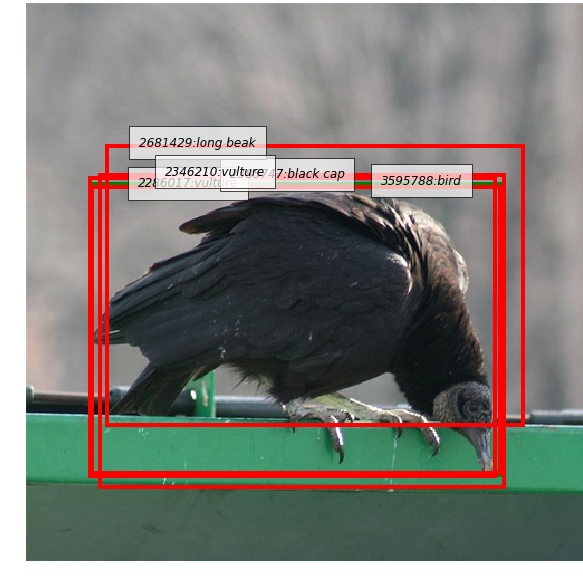
\includegraphics[scale=0.4]{figures/vulture.png} 
\begin{tabular}{lp{6cm}}
object id & linked region descriptions\\
\hline
3595788 & the \textbf{bird} is black in color, nose of the \textbf{bird}, a \textbf{bird} relaxing in stand, small white beak of \textbf{bird}, large black talon of \textbf{bird}, a \textbf{bird} on a green pole, a green bar under \textbf{bird}, black \textbf{bird} on green rail, small black eye of \textbf{bird}\\
2286017 & large black \textbf{vulture} on fence, a vulture on bar\\
2385747 & small white beak of \textbf{bird}\\
2681429 & a semi \textbf{long beak}\\  
2346210 & a black and gray \textbf{vulture}\\
 \end{tabular}
\caption{Bounding boxes, names and region descriptions for an object in VisualGenome}
\label{fig:bird}
\end{center}
\end{figure}

\vg \cite{krishna2016visualgenome} is one of the most densely and richly annotated resources currently available in L\&V; below, we focus on aspects immediately relevant to object naming.
%In the following, we will focus on describing aspects immediately relevant to object naming only, but many other annotations are available as well (e.g. questions, paragraphs, etc.)
%\paragraph{Collection and annotation procedure}
\vg aims at providing a full set of descriptions of the scenes which images depict in order to spur complete scene understanding. 
The data collection followed a complex procedure, involving many different rounds of annotation.
The first round of the procedure, and the basic backbone for the further rounds, is a collection of region-based descriptions: workers were asked to describe regions in the image and draw boxes around the corresponding area in the image (for examples, see Figure \ref{fig:bird}).

In a second, independent round (involving new workers), annotators were asked to process the region descriptions by (i) marking the object names contained in the region description, and (ii) drawing a tight box around the corresponding region. As different region descriptions can potentially mention the same objects, each worker was shown a list of previously marked objects and encouraged to select on existing object rather than annotating a new one.

\gbt{@Sina, pls check that I got this right:}
One of the main advantages of \vg are its size, with 3.8 million objects as opposed to 50K and 243K for the other two datasets, and its category coverage, with a vocabulary of object names of 105K compared to 5K/10K.
Another is the fact that it potentially provides exhaustive annotations of objects in the image, often with several region descriptions and possibly object names per object.
This should make it easier to identify factors intervening in naming choices.
However, there is a crucial pitfall: As Figure \ref{fig:bird} shows, there is only a partial linking of objects that are mentioned across different region descriptions; for instance, the first, second, and fifth object IDs in the figure actually correspond to the same object.
Moreover, the regions for the beak of the object (third and fourth object IDs) overlap with those of the bird.
This means that the identity of objects cannot be established based on the annotation, which severely limits the usefulness of the annotations.

\subsection{Discussion}

\gbt{Do we need a discussion section wrapping up what we've said in this survey section and motivating MN?}

As the discussion above showed, while some existing resources can be used to shed light on factors affecting naming choices, they do not provide enough data to assess \textbf{naming variation}, which requires having data from many subjects.
This is the motivation for our dataset, ManyNames, an augmentation of \vg.

%%% Local Variables:
%%% mode: latex
%%% TeX-master: "lrec2020naming"
%%% End:


\section{A New Dataset: ManyNames}
\label{sec:data}
% Number of images/objects:        25,596\\
% Number of object names:  450\\
% Number of collection nodes (synsets):    52 \\

\begin{table*}[htp]
	\small
	\centering
	\begin{tabular}{lp{14cm}}
			\toprule
			Domain & \multicolumn{1}{c}{Collection synsets}\\
			\midrule			
			animals\_plants & ungulate$_1$ (2037), horse$_1$ (833), feline$_1$ (763), dog$_1$ (688)
			bird$_1$ (389), flower$_1$ (44), rodent$_1$ (27), insect$_1$ (12), fish$_1$ (11)\\
			buildings      &  house$_1$ (364), bridge$_1$ (297), shelter$_1$ (169), restaurant$_1$ (58),
                                         outbuilding$_1$ (31), hotel$_1$ (19), housing$_1$ (17), place\_of\_worship$_1$ (12)     \\
			clothing       &  shirt$_1$ (968), overgarment$_1$ (786), dress$_1$ (199), headdress$_1$ (135),
                                         neckwear$_1$ (65), robe$_1$ (27), glove$_2$ (7), footwear$_1$ (5)    \\
			food           &  dish$_2$ (812), baked\_goods$_1$ (770), foodstuff$_2$ (280), vegetable$_1$ (48),
                                         edible\_fruit$_1$ (42), beverage$_1$ (23)   \\
			home           &  furnishing$_2$ (5,355), vessel$_3$ (525), kitchen\_utensil$_1$ (132), crockery$_1$ (92),
			cutlery$_2$ (82), tool$_1$ (72), lamp$_1$ (34)    \\
			people         & woman$_1$ (1768), man$_1$ (1167), male\_child$_1$ (853), athlete$_1$ (396),
			 child$_1$ (333), creator$_2$ (11), professional$_1$ (5)    \\
			vehicles       &  aircraft$_1$ (1208), train$_1$ (957), car$_1$ (727), motorcycle$_1$ (564),
                                         truck$_1$ (559), boat$_1$ (499), ship$_1$ (38)    \\
			\bottomrule
		\end{tabular}
		\caption{Overview of the ManyNames dataset: Synset nodes for each domain (subscript indicates synset number; number of instances in parentheses).
                  \label{tab:overview_dataset2}}
	\end{table*}

\begin{table*}[htp]
	\small
	\centering
	\begin{tabular}{@{~}l@{~}l@{~}l@{~}l@{~}l@{~}l@{~}l}
		\toprule
		vehicles &            food & animals\_plants &           home &        buildings &             people &      clothing \\
		\midrule
		train (954) &  pizza (518) &  giraffe (915) &  bed (888) &  house (340) &  boy (853) &  shirt (904) \\
		car (642) &  cake (261) &  horse (822) &  bench (714) &  bridge (274) &  man (806) &  jacket (451) \\
		plane (485) &  bread (186) &  cat (754) &  table (687) &  dugout (91) &  woman (766) &  coat (267) \\
		airplane (479) &  sandwich (153) &  dog (654) &  desk (672) &  tent (53) &  girl (650) &  dress (190) \\
		motorcycle (466) &  bun (143) &  zebra (461) &  counter (516) &  restaurant (33) &  lady (342) &  hat (77) \\
		% truck (465) &  cheese (110) &  cow (324) &  couch (366) &  overpass (23) &  guy (330) &  t-shirt (62) \\
		% boat (450) &  donut (78) &  bird (295) &  chair (365) &  grill (22) &  child (230) &  tie (51) \\
		% jet (106) &  salad (70) &  sheep (216) &  carpet (307) &  garage (18) &  batter (110) &  blazer (43) \\
		% aircraft (85) &  sauce (68) &  bull (48) &  bowl (219) &  hotel (16) &  kid (85) &  hood (26) \\
		% van (76) &  apple (33) &  flower (40) &  curtain (182) &  castle (14) &  skateboarder (80) &  cap (20) \\
		\bottomrule
	\end{tabular}
	\caption{Overview of the ManyNames dataset: Top 5 VG names for each domain (number of instances in parentheses).\label{tab:overview_dataset1}}
\end{table*}

\begin{figure*}[htp]
  \centering
  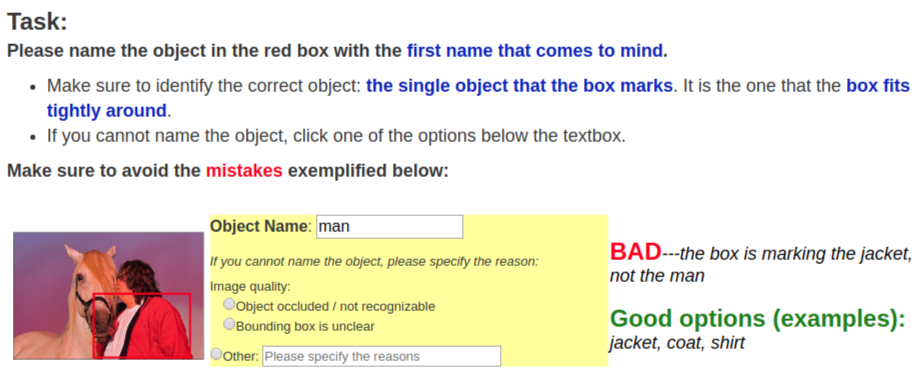
\includegraphics[width=1.5\columnwidth]{figures/round0_cropped.png}
  \caption{Instructions for AMT annotators for the first round (whole instructions showed more examples, see Figure~\ref{fig:instructions2}).}
  \label{fig:instructions1}
\end{figure*}

We take data from \vgenome~(VG, \newcite{krishna2016visualgenome}), which
contains a dense region-based labeling of $108$K~images with, inter alia, object names, attributes and relationships,
all linked to WordNet synsets \cite{fellbaum1998wordnet}.
\vg suits our purpose of collecting names for naturalistic instances of common objects, as it has images of varying complexity, with close-ups as well as images with many objects.
As common in Computer Vision, objects are localized as bounding boxes, as in Figure~\ref{fig:cake}.% 
\footnote{We use image and object interchangeably in the following, since we only selected one target object per image (i.e., each object and image in VG is chosen at most once).}

\subsection{Sampling of Instances}
\label{ssec:sampling}

%Criteria: From CV: select images depicting objects with relatively frequent names; From CogSci: select objects which have been frequently studied in cognitive science/psychological norming studies; we chose McRae et al. as basis.
We selected images from seven domains: \domain{animals\_plants}, \domain{buildings}, \domain{clothing}, \domain{food}, \domain{home}, \domain{people}, \domain{vehicles}. 
They are all based on McRae et al.'s  \cite{mcrae2005semantic} feature norms, a dataset widely used in Psycholinguistics that comprises common objects of different categories, except for \domain{people}, which we added because it is a very frequent category in \vg and a very prominent category for humans.
% We start from the concepts of McRae et al.'s feature norms (REF), which are common objects of different categories (e.g.,~\domain{animals}, \domain{furniture}) and, as such, have a high overlap with standard datasets of object norming studies (REFS).
% We added the \domain{person} category because it is very frequent category in \vgenome.

Within each domain, we aimed at collecting instances at different taxonomic levels to cover a wide range of phenomena, but this is not straightforward because ontological taxonomies do not align well with the lexicon (for instance, \textit{dog} and \textit{cow} are both mammals, but \textit{dog} has many more common subcategories), and most domains are not organized in a clear taxonomy in the first place (e.g.\ \domain{home}).
Instead, we defined a set of synsets ($52$\ in total; listed in Table~\ref{tab:overview_dataset2}) that we used to collect object instances from \vg, as follows. 

First, to create our synset set, we chose those \vg synsets that match or subsume the object classes in the McRae norms, and have a high number of \vg object instances of different names.\cs{prev. sentence this is still a bit fluffy}
For example, \vg instances subsumed by McRae's \textsl{dog} were named \textsl{beagle, greyhound, puppy, bulldog}, etc., while McRae's \textsl{duck}, \textsl{goose}, or \textsl{gull} did not have name variants in \vg, so we kept \textsl{dog} and \textsl{bird} (which subsumes \textsl{duck}, \textsl{goose}, or \textsl{gull}) as collection synsets.
%\gbt{Just to clarify: we also collected objects named \textsl{duck}, \textsl{goose}, or \textsl{gull}, right? Not only \textsl{bird}?}

We then retrieved all VG images depicting an object whose name matches or is subsumed by words in one of these synsets; we refer to these words as \textit{seeds} ($450$\ in total).
\gbt{from the dataframe in the github it's 449. Also, there are some mistakes in the list of seeds ('dugout.', 'man's') -- to check after the deadline.}
We did not consider objects with names in plural form, with parts-of-speech other than nouns\footnote{We obtained tags with CoreNLP \cite{manning2014stanford}.}, or that were multi-word expressions (e.g.,~\textsl{pink bird}). 
We further only considered objects whose bounding box covered~\mbox{$20-90\%$} of the image area.
% We based the definition of our set of nodes on the WN (REF) synsets of the McRae concepts (e.g.,~dog, duck, goose, gull), the nominal WordNet hierarchy, and the frequency distribution of the VG object names' synsets.\footnote{TODO: need to be clear from the general description of VG that the frequ. of instances labeled with the synset of the object name is meant.} 
% First, we selected a set of collection node candidates---synsets which match (e.g.,~\textsl{dog, duck, goose, gull}) or subsume (e.g.,~\textsl{mammal, bird}) the McRae synsets\footnote{Specific synset IDs, e.g.,~dog.n.01, are omitted for readability.}. 
% From these candidates we kept those as collection nodes which had a high frequency of VG object instances of different names. For example, VG instances  subsumed by McRae's \textsl{dog} were named \textsl{beagle, greyhound, puppy, bulldog}, etc., while McRae's \textsl{duck, goose}, or \textsl{gull} did not have name variants in VG, so we kept \textsl{dog} and \textsl{bird} as collection nodes.
%\paragraph{Collection of instance candidates}
% Goal of above procedure was the collection of instances of selected object classes---our nodes--- whose VG names correspond to or subsume (are hypernyms of) a McRae concept, and whose object names differ, that is, of which we can expect that people possess different names for them (e.g.,~\textsl{duck, goose, gull} for \textsl{bird}).
% \paragraph{Sampling of instances}
Because of the Zipfian distribution of names, and to balance the collection, we sampled instances depending on the size of the seeds: up to $500$\ instances for seeds with up to $800$\ objects, and up to $1000$\ instances for larger seeds. This yielded a dataset of\ $31,093$~instances, which was further pruned during annotation, as explained next.
Table~\ref{tab:overview_dataset1} shows the top 5 \vg names in each of the domains.

\subsection{Elicitation Procedure}
\label{ssec:elicitation}

To elicit object names, we set up a crowdsourcing task on Amazon Mechanical Turk (AMT).
In initial pilot studies, we found object identification via bounding boxes to be problematic.
In some cases, the bounding box was not clear; in others, AMT workers named objects that were more salient than the one signaled by the box (for instance, for a box around a jacket, the man wearing it).
We took special care of minimizing this issue in two ways: Specifying the instructions such that workers pay close attention to what object is being indicated in the box, and pruning images with unclear boxes or occluded objects via an initial collection round in which we allowed workers to mark such cases.
Figure~\ref{fig:instructions1} shows the task instructions for this first round, in which 9 workers annotated each image.

%We eliminated around $5.5$K\ images based on pruning, obtaining the final dataset with $25,596$\ images.
After the first round, and based on the opt-out annotation, we kept images that met all the following conditions (thresholds were estimated via manual inspection): (i) they were not marked as occluded by any subject; (ii) ``Bounding box is unclear'' was marked at most twice; (iii) at most 17\% of elicited names were in plural form (to remove cases where the bounding box contains several objects); (iv) the most frequent elicited name is of the same domain as the \vg name.
This yielded $25,596$ images (we discarded $5,497$).
We then did 3 more collection rounds, obtaining a total of 36 images per object.
Figure~\ref{fig:instructions2} shows the instructions for these rounds; they were accompanied by a FAQ solving common issues. 
We shuffled the set of images per task between rounds, and workers could only participate in one round, to avoid workers annotating an instance more than once.
Overall $841$\ workers took part in the data elicitation, with a median of  $261$\ instances \mbox{($\textrm{range}=[9,17K]$)} per worker.

\begin{figure*}[htp]
  \centering
  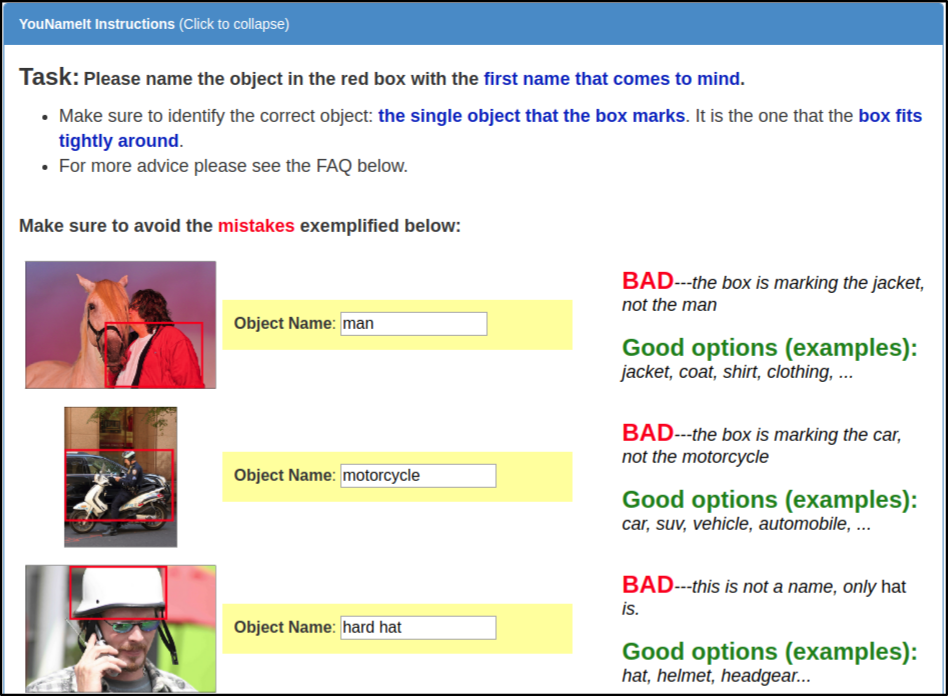
\includegraphics[width=1.5\columnwidth]{figures/round1+_p1.png}
  \caption{Instructions for AMT annotators for rounds~$2$ to~$4$.}% They were accompanied by the FAQ in Figure~\ref{fig:faq}}
  \label{fig:instructions2}
\end{figure*}

% \begin{figure*}[htp]
%   \centering
%   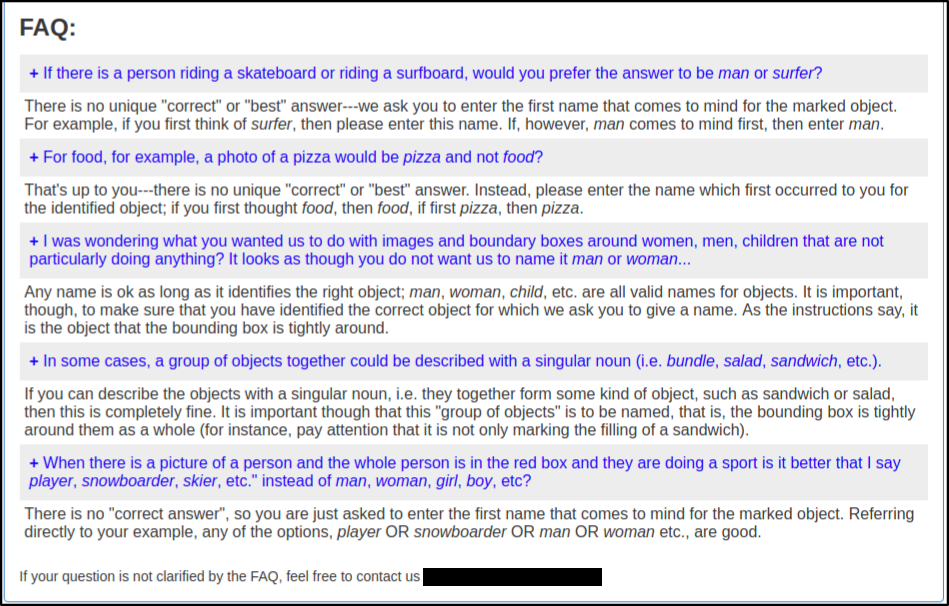
\includegraphics[width=1.5\columnwidth]{figures/round1+_p2.png}
%   \caption{FAQ accompanying the instructions for AMT annotators for rounds~$2$ to~$4$.}
%   \label{fig:faq}
% \end{figure*}

%\cs{Maybe say something about the rejections, if space permits it.}

%%% Local Variables:
%%% mode: latex
%%% TeX-master: "lrec2020naming"
%%% End:



	
\section{Analysis}
\label{sec:analysis}
%\gbt{Points to discuss in the paper, as discussed with Carina May 16:}
%
%\begin{itemize}
%\item Super high variance in the agreement. Higher agreement for instances, lower for classes. Suggests systematicities at the instance level that do not depend on the class. Hypothesis, supported by qualitative analysis (Figure 3): relevance of visual perceptual factors. E.g.: saliency, background/foreground (desk-keyboard; bridge-train); ``angle'' from which the object is shown (see girl-t-shirt example); \dots In addition, we also find aspects discussed by Psycholing, but at the level of the instance: Typicality (see truck-bus example, bridge-dock, bench-seat). 
%\item Forget about WordNet.
%\item Implications for lang\&vision: 1) synset classification won't do (if the goal is to predict/label an object); 2) name classification won't do either; 3) ``mistakes'' done by models are also done by humans -- role of referential uncertainty.
%\end{itemize}


In this section, we investigate to what extent names annotated in VisualGenome and elicited in ManyNames can be considered canonical, i.e. to what extent speakers agree in their naming choices.
Whereas traditional picture naming studies typically use a prototypical image per category (see Figure~\ref{fig:picture_naming}) and, hence, are mostly interested in the agreement on concept or category-level, we carry out an analysis on two different levels: First, we will look at instances and see to what extent names overlap for the same object. 
Second, we will use the existing annotation of names in VisualGenome to analyze agreement on the level of classes.
\begin{figure}[t]
	\centering
	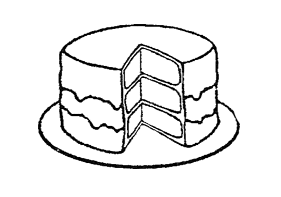
\includegraphics[scale=.5]{figures/snodgrass_vanderwart_cake_042.png}
	\caption{Example of a picture of \textsl{cake} used in traditional picture naming studies (REF to Vanderwart \& Snodgrass) \label{fig:picture_naming}}
\end{figure}

\subsection{Names, instances, classes}

First of all, to see whether objects in ManyNames bear a canonical name, we simply count how many different names (i.e.\ types) are given to instances, and to all instances that have the same synset annotated in VisualGenome. 
As the data is collected via crowdsourcing and a certain amount of noise is to be expected, we apply different frequency thresholds on the response sets for instances and synsets.
Figure \ref{fig:ntypes} shows the cumulative histograms for type counts, obtained with different thresholds (from 1 to 6).
Without any frequency thresholding, the proportion of instances and classes that have a single name annotated is small, i.e.\ below 10\% in both cases. When raising the threshold up to a minimum of 4 occurences in the response set  for instances (meaning more than 10\% of the 36 annotations), the proportion of objects that really only have a single name annotated is considerably higher, but still below 50\%.
Thus, as expected in a free annotation scenario, the MN data contains a certain number of low-frequency responses.
The fact that even after applying a relatively strict frequency filter most objects have more than one name annotated indicates that there is a non-negligible  level of variation when different speakers name the same object.

The amount of variation increases substantially when looking at the number of names we find for different synsets in Visual Genome, as is indicated by the histogram for type counts of synsets in Figure \ref{fig:ntypes}.
Here, we observe that the rise of the curve is much less steep than for instances and, generally, there are many synsets with more than 10 or even 20 different name types, even after applying the frequency threshols.

\begin{figure*}
\begin{minipage}[b]{0.4\linewidth}
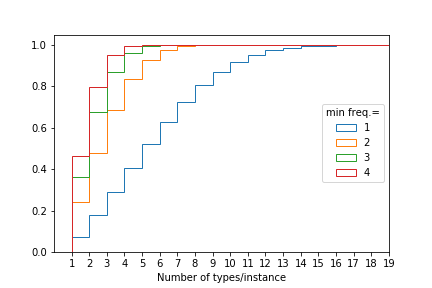
\includegraphics[scale=.4]{Figures/types_instances.png}
\end{minipage}
\begin{minipage}[b]{0.6\linewidth}
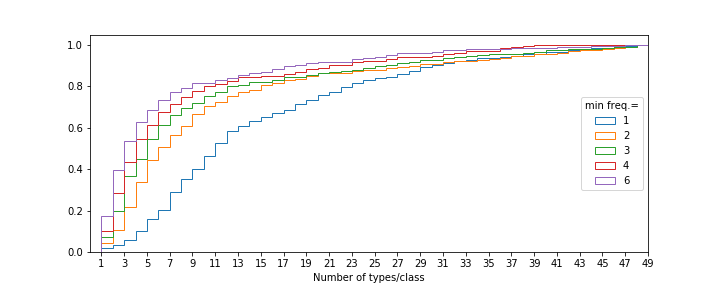
\includegraphics[scale=.4]{Figures/types_classes.png}
\end{minipage}
 \caption{\label{fig:ntypes} Cumulative histograms for number of types found for instances and classes, based on different frequency tresholds (applied on the level of instances and classes respectively)}
\end{figure*}


\subsection{Agreement}

We compute the following agreement measures:

\begin{itemize}
\item \textbf{\% top}: the average relative frequency of the most frequent response (shown in percent)
\item \textbf{$H$}: the $H$ agreement measure used previously in the psycholinguistic literature
\cs{How is this defined?}
\begin{equation}
H = \sum_{i=1}^k p_i\ log_2(1/p_i)
\end{equation}

\item \textbf{N}: the average number of types in the response set of ManyNames
%\item \textbf{N$_{>1}$}: the average number of types, excluding types that have been annotated only once
\cs{alternatively we could show a plot going from 1 to, let's say, $>10$}
\item \textbf{top=VG}: the proportion of items where the top response in ManyNames corresponds to the VisualGenome name
\item \textbf{\% VG}: the average relative frequency of the VisualGenome name in the response set

\end{itemize}

For measuring \textbf{instance-level agreement}, we consider all names annotated for an object as a response set and then average over these response sets. Furthermore, we compute \textbf{class-level agreement} by merging the response sets for all objects that have the same synset (given for the original VisualGenome name) and compute the measures over these aggregated response sets.
\gbt{@Sina, what are the synsets that you got here? Are they collection nodes, or the synset of the VG name as annotated in VG?}


Table \ref{tab:agree} shows the analysis of the instance-level and category-level agreement.
On the instance-level, our annotators achieve a fair amount of overlap in their object naming choices. 
Thus, for roughly 70\% of our objects (\textbf{std=?}), the most frequent response in ManyNames corresponds to the original VisualGenome name and, similarly, the average frequency of the top response is also 70\%. 
%Generally, this seems to suggest that indeed many objects in our data set have a canonical name. 
\sz{For NLP people, this looks like a good agreement (given that people were free to type what they wanted). For vision people who might think of it as an object labeling task, this would be pretty low/bad agreement.}
At the same time, the average number of name types per object (5.7, or 2.9 when excluding low-frequency types in each response set) suggests that there is a stable amount of naming variants that is elicited for instances. 
Furthermore, the agreement varies quite considerably among domains \cs{refer to std}:  in the animal domain, which is often discussed in the object naming literature, annotators achieve a very stable and robust agreement of over 90\% and an $H$ agreement which comes close to 0 (where 0 is perfect agreement). 
The people domain, on the other hand, is subject to much more variation and agreement is dramatically lower here, and comes close to 50\% for \% top.



%\gbt{Super-interesting results.}
Finally, the category-level agreement figures tell yet another story: when aggregating the responses for all objects with the same VisualGenome synset, we obtain on average 30 types (with $N_{>1})$, i.e. variants of the original VG class. 
Surprisingly, here, only 32.7\% of the aggregated response sets still have the VG name as the most frequent response, which means that for 70\% of the VG names, annotators in ManyNames, on average, prefer a different name.  
Likewise, the relative frequency of the top response drops considerably and $H$ increases from 1.3 for instance-level agreement to 2.4 on object-level agreement.  
%\cs{Can we say more about what's going on in the people and vehicles domain, category-level, top=VG? E.g., put corresponding examples in Tab.\ref{tab:qual}}
%

\subsection{Variation and WordNet}

Previous work on large-scale collections of labels or names of objects has (explicitly or implicitly) assumed that once naming data is canonical, linguistic alternatives of the canonical name can simply be retrieved from existing taxonomies like e.g.\ WordNet. 
%If this was indeed the case, it would be feasible (and probably even desirable) to canonicalize object names during dataset collection, without loosing too much information about linguistic variations in natural object naming scenarios (like e.g.\ referring expression generation).
Hence, in this section, we investigate to what extent the variation in object naming that we find in our MN data set (see previous Section) is covered by WordNet.
%In this section, we take a closer look at the lexical variation we observe in our data set. 
We analyze the data points where participants attributed different names to the same object and extract a set of  pairwise \textbf{naming variants}. These naming variants correspond to pairs of words that can be used interchangeably to name certain objects.
For each object, we extract the set of naming variants $s = \{ (w_{top},w_2), (w_{top},w_3), (w_{top},w_4),... \}$  where $w_{top}$ is the most frequent name annotated for the object and $w_2 ... w_n$ constitute the less frequent alternatives of $w_{top}$.  The  \textbf{type frequency} of a naming variant $(w_{top},w_x)$ corresponds to the number of objects where this variant occurs. The \textbf{token frequency} of $(w_{top},w_x)$ corresponds the count of all annotations where $w_x$ has been used instead of $w_{top}$.
In Table \ref{tab:exvariants}, we show the naming variants with the highest raw token frequency for each domain. 
The naming variants can be grouped according to their lexical relation, as follows:

\begin{itemize}
\item \textbf{synonymy}: e.g.\ aircraft vs. airplane 
\item \textbf{hyponymy}: e.g.\ man vs. person
\item \textbf{co-hyponymy}: e.g.\ swan vs. goose
\item \textbf{no relation}: e.g.\  desk vs. apple
\end{itemize}

\begin{table}
\small
\centering
\begin{tabular}{lcc}
\toprule
         relation & \% types & \% token \\
\midrule
% meronym &  0.1 &  0.2 \\
% holonym &  0.1 &  0.4 \\
 synonym &  1.1 &  1.1 \\
 hyponym &  2.2 &  3.8 \\
 co-hyponym &  3.1 &  5.9 \\
 hypernym &  10.5 &  27.7 \\
 word-not-covered &  10.6 &  2.6 \\
 rel-not-covered &  72.2 &  58.3 \\
\bottomrule
\end{tabular}
\caption{Lexical relations of naming variants in MN to annotated VG synset, averaged over synsets}
\label{tab:rel}
\end{table}


Research on object naming following the idea of entry-level categories has, essentially, exclusively looked at names that stand in a hierarchical relation (i.e.\ hyponymy/hypernymy).

We use WordNet to extract lexical relations between the naming variants in our data set.
Unfortunately, this means that we have to exclude a certain portion of the data as either (i) one of the name is not covered in WordNet, (ii) we cannot find a lexical relation between the two names (see below). Also, we had to be relatively permissive with respect to the definition of hyponymy/co-hyponymy. 
For instance, to analyze \textit{giraffe} as a hyponym of \textit{animal} we have to look at the closure of the hyponyms of \textit{animal} with a depth of 8 (in WordNet).
\sz{should we call this co-hyponymy or co-hierarchical relation?}

\sz{include Table that reports counts of the naming variants, coverage in WordNet etc.} \gbt{I think it'd be best to put the out-of-wordnet info in the Lexical relations table -- this way we have everything in one place.}

Table \ref{tab:rel} shows the distribution of lexical relations for those naming variants that we were able to analyze with WordNet.
Both in terms of their types and token frequency, the naming variants that instantiate a (loose) co-hyponymy relation are by far the most frequent.
\sz{discuss in more detail, discuss: to what extent is this an artefact of WordNet?}
This is really interesting: most research on object naming, to date, has focussed on hyponymy/hypernymy, i.e. variation that relates to hierarchical relations between object names.
Our data suggests that co-hierarchical variation is really important too.



%\subsection{Qualitative Analysis}

%\sz{put qualititative discussion here} Table \ref{tab:qual} shows examples for canonical and non-canonical VG names in our data set, where canonical means that the name was the top response in the aggregated response set in ManyNames.

%\begin{table}
%\small
%\begin{tabular}{lp{4.8cm}r}
%\toprule
%VG name &  top5 MN names &  n$_{obj}$  \\
%\midrule
%\multicolumn{3}{c}{\it Canonical VG names with max agreement in MN}\\
% giraffe &  giraffe (96.8), animal (1.2), zebra (0.4), camel (0.3), pole (0.1) &  915 \\
% zebra &  zebra (96.3), animal (1.0), giraffe (0.9), horse (0.2), microwave (0.2) &  461  \\
% cat &  cat (94.8), animal (0.9), kitten (0.8), dog (0.4), laptop (0.2) &  754\\
%\midrule
%\multicolumn{3}{c}{\it Canonical VG names with min agreement in MN}\\
% booth &  booth (19.3), table (12.3), phone booth (9.8), bench (6.7), building (4.4) &  11 \\
% cabbage &  cabbage (21.4), lettuce (17.0), hotdog (11.9), food (10.7), salad (10.4) &  9 \\
% robe &  robe (22.1), shirt (16.8), jacket (13.3), dress (5.7), clothing (3.2) &  19 \\
%  \midrule
%  \multicolumn{3}{c}{\it Non-canon. VG names with max agreement in MN}\\
% sedan &  car (88.4), wheel (3.1), vehicle (2.3), automobile (1.3), dog (0.8) &  11 \\
% pony &  horse (83.9), pony (9.1), animal (2.9), donkey (1.1), cow (1.1) &  8 \\
% necktie &  tie (81.4), necktie (10.2), shirt (4.6), ties (1.5), jacket (0.5) &  11 \\
% \midrule
%   \multicolumn{3}{c}{\it Non-canon. VG names with min agreement in MN}\\
% shelter &  umbrella (9.7), shelter (8.8), roof (8.0), tent (7.1), building (6.8) &  10 \\
% bath &  shower (13.3), elephant (9.9), birdbath (8.1), water (7.2), trough (7.2) &  10 \\
% vegetable &  food (15.7), broccoli (13.1), sandwich (10.6), salad (9.3), pizza (7.8) &  25 \\
%\bottomrule
%\end{tabular}
%\caption{Examples for VisualGenome (VG) names and their most frequent corresponding responses in ManyNames (MN; percentages shown in brackets). ``Canonical'' means that the VG name is the top name in MN, and non-canonical vice versa.}
%\label{tab:qual}
%\end{table}

\begin{figure*}
\begin{minipage}[b]{0.5\linewidth}
{\footnotesize
\setlength{\tabcolsep}{1pt}
\begin{tabular}{p{4cm}|p{4cm}|p{4cm}|p{4cm}}
%\textbf{desk} &  \raisebox{-\totalheight}{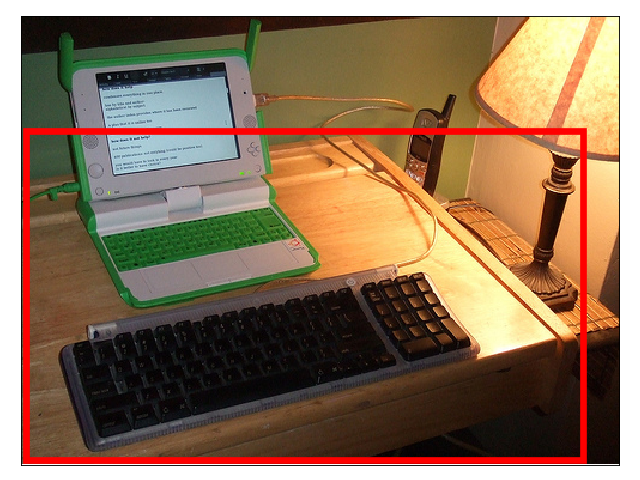
\includegraphics[width=0.9\linewidth]{figures/2320949_1048853_singleton_obj.png}} MN: keyboard  &
%\raisebox{-\totalheight}{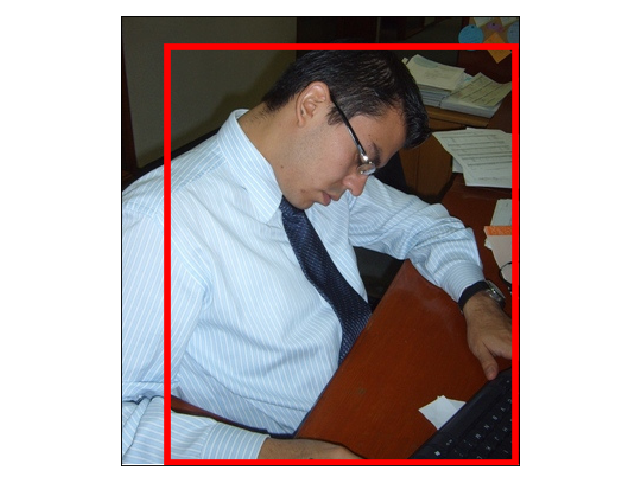
\includegraphics[width=0.9\linewidth]{figures/2343219_926143_supercat_unique.png}}  MN: desktop &
%\raisebox{-\totalheight}{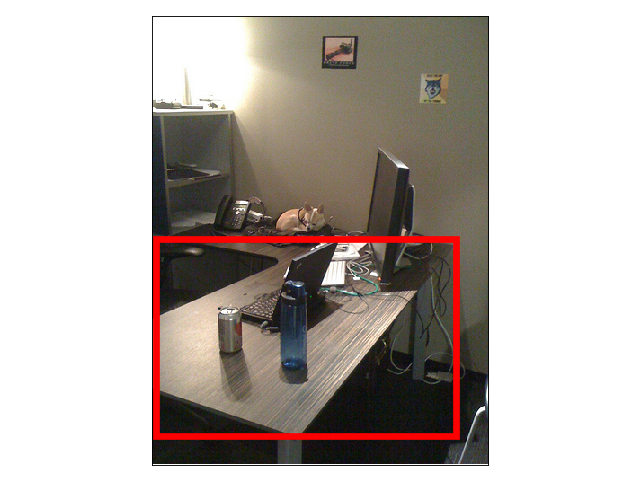
\includegraphics[width=0.9\linewidth]{figures/2354847_1742687_seed_ambiguous.png}} MN: computer \\
%\textbf{bench} &  \raisebox{-\totalheight}{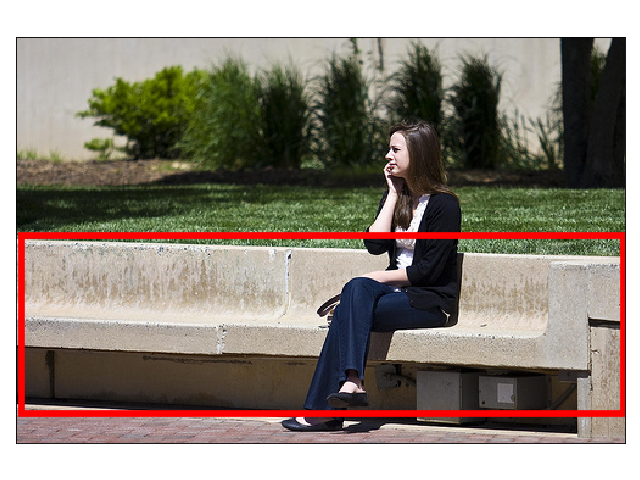
\includegraphics[width=0.9\linewidth]{figures/2350360_1042111_supercat_unique.png}} MN: table  &
%\raisebox{-\totalheight}{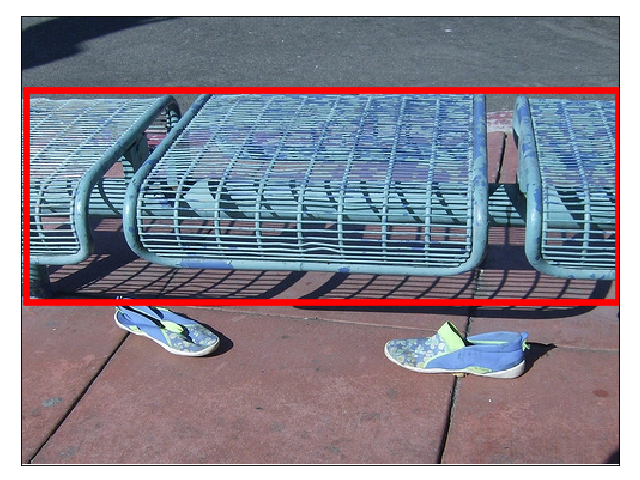
\includegraphics[width=0.9\linewidth]{figures/2389358_1261752_singleton_obj.png}}  MN: seat &
%\raisebox{-\totalheight}{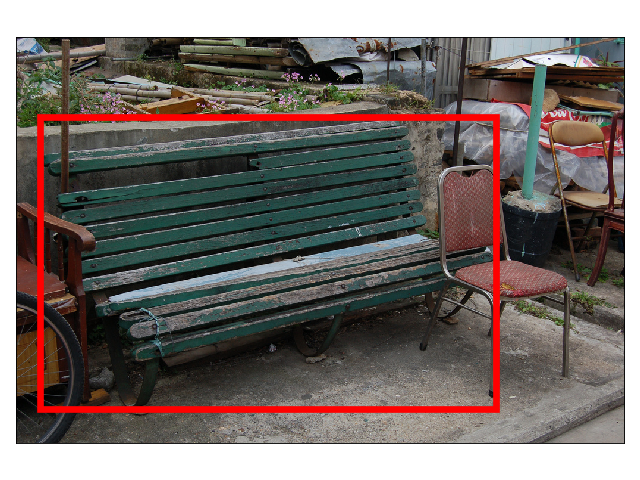
\includegraphics[width=0.9\linewidth]{figures/1593011_2063521_singleton_obj.png}} MN: wood \\
\multicolumn{4}{c}{\textbf{VG: sandwich}}\\
 \raisebox{-\totalheight}{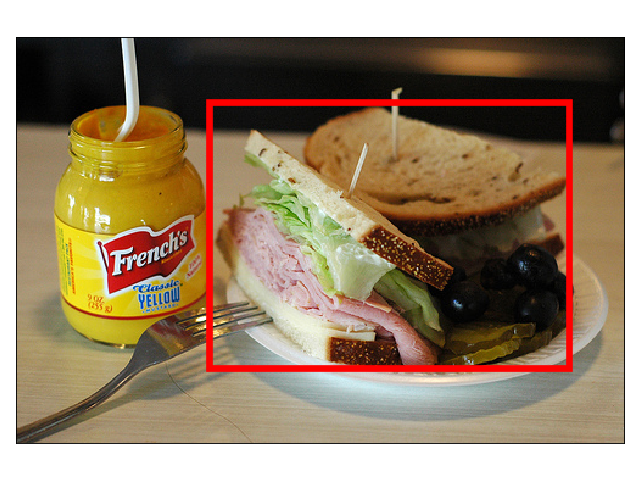
\includegraphics[width=0.9\linewidth]{figures/2339876_3928476_supercat_unique.png}} sandwich (34) &
\raisebox{-\totalheight}{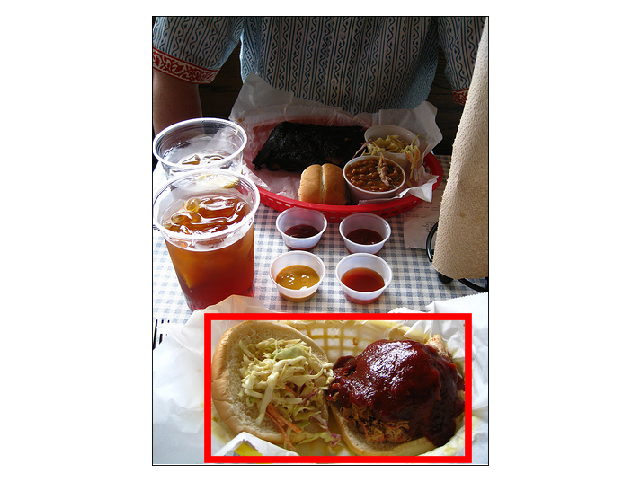
\includegraphics[width=0.9\linewidth]{figures/2379889_1353176_supercat_unique.png}}  sandwich (15), basket (6), food (5), burger (2), hamburger (2), meal (2) &
\raisebox{-\totalheight}{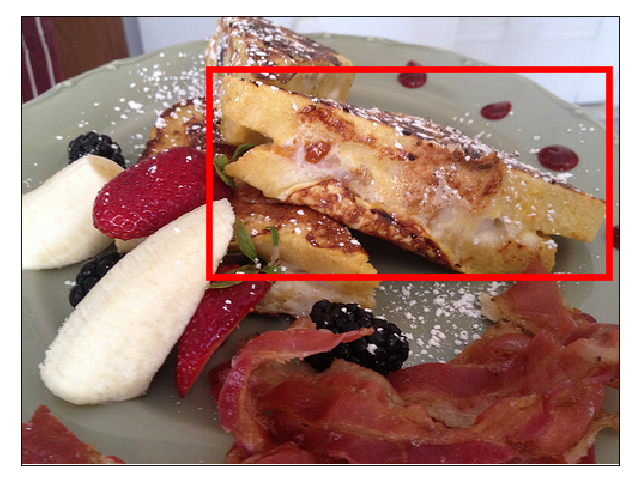
\includegraphics[width=0.9\linewidth]{figures/2394266_465678_singleton_obj.png}} food (10), sandwich (8), toast (5), french toast (4), dessert (2), breakfast (2) &
\raisebox{-\totalheight}{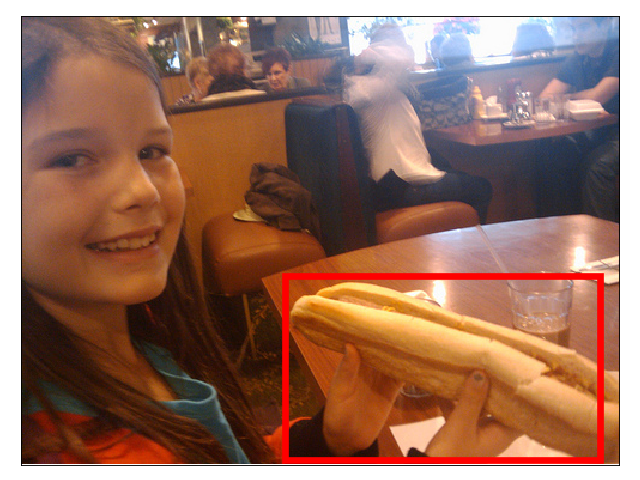
\includegraphics[width=0.9\linewidth]{figures/2386509_681763_supercat_unique.png}} hotdog (14), food (7), bun (4), sandwich (3), bread (2)\\ 
\multicolumn{4}{c}{\textbf{VG: bridge} }\\ 
\raisebox{-\totalheight}{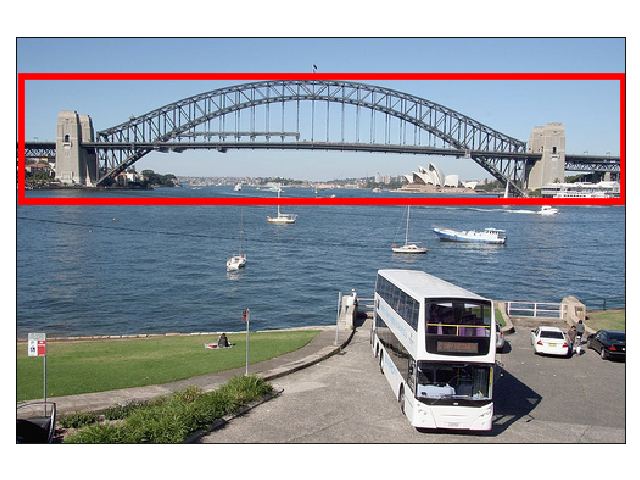
\includegraphics[width=0.9\linewidth]{figures/2341667_2006329_singleton_obj.png}} bridge (35)  &
\raisebox{-\totalheight}{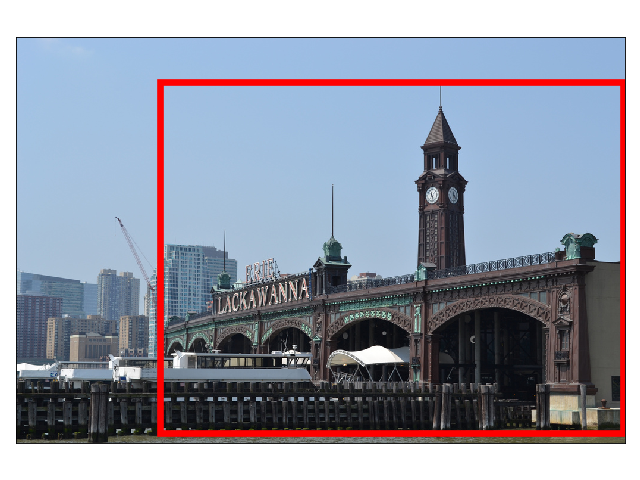
\includegraphics[width=0.9\linewidth]{figures/1592509_1610006_singleton_obj.png}} bridge (20), building (11)  &
\raisebox{-\totalheight}{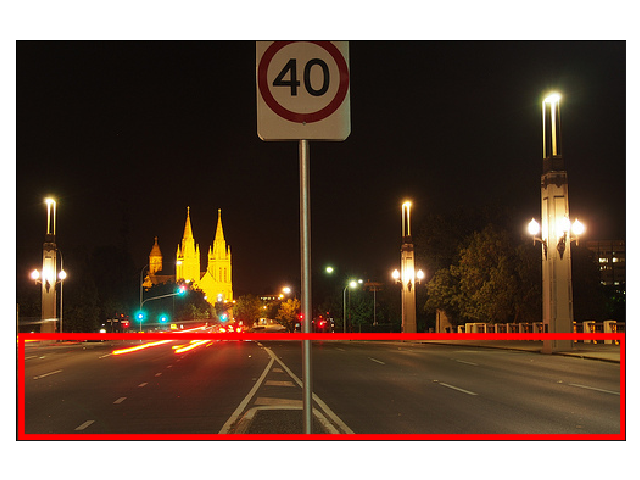
\includegraphics[width=0.9\linewidth]{figures/2384683_1306430_singleton_obj.png}} street (16), road (15), bridge (3) &
\raisebox{-\totalheight}{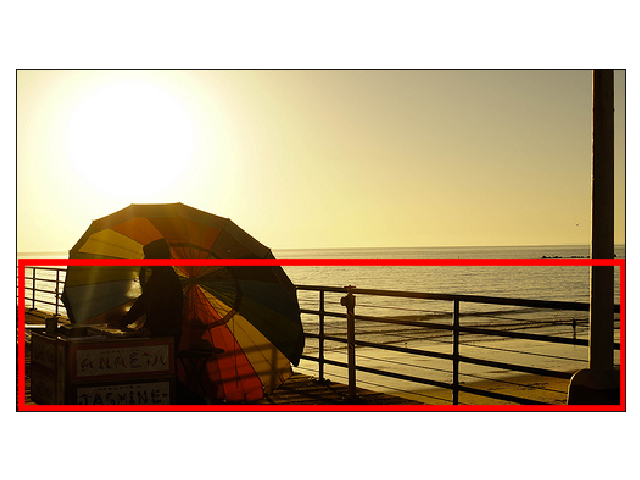
\includegraphics[width=0.9\linewidth]{figures/2412972_3494120_singleton_obj.png}} pier (6), railing (5), dock (5), bridge (5), fence (4), rail (3), boardwalk (3)\\ 
\multicolumn{4}{c}{\textbf{VG: bed}}\\ 
\raisebox{-\totalheight}{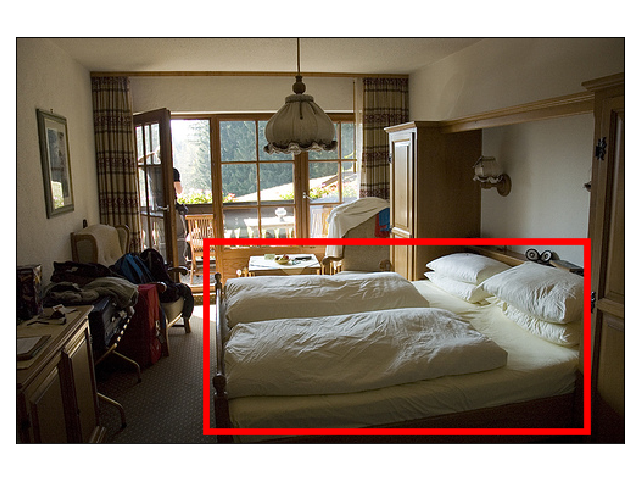
\includegraphics[width=0.9\linewidth]{figures/2321254_3438076_singleton_obj.png}} bed (36)  &
\raisebox{-\totalheight}{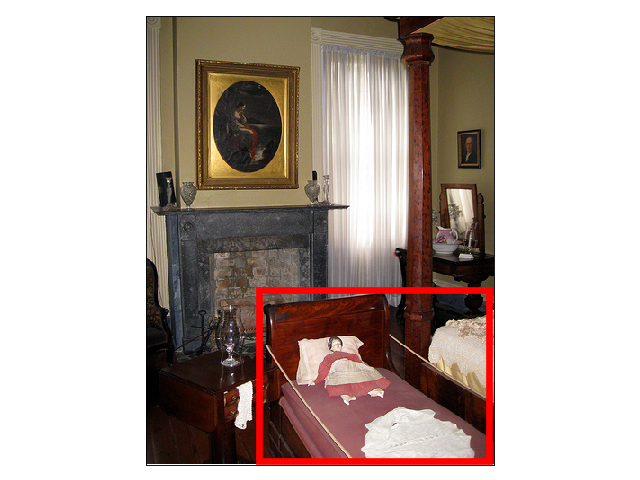
\includegraphics[width=0.9\linewidth]{figures/2324306_3412337_singleton_obj.png}}  bed (16), bench (6), crib (5) &
\raisebox{-\totalheight}{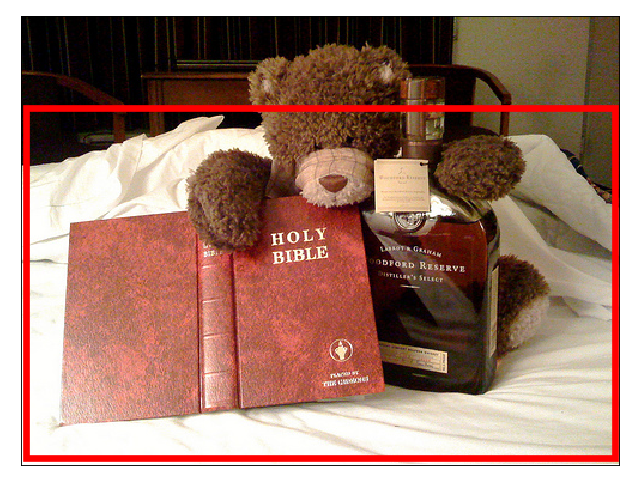
\includegraphics[width=0.9\linewidth]{figures/2342811_3485104_singleton_obj.png}}  bed (17), book (6), table (4), toy (3), bible (2), doll (2) & 
\raisebox{-\totalheight}{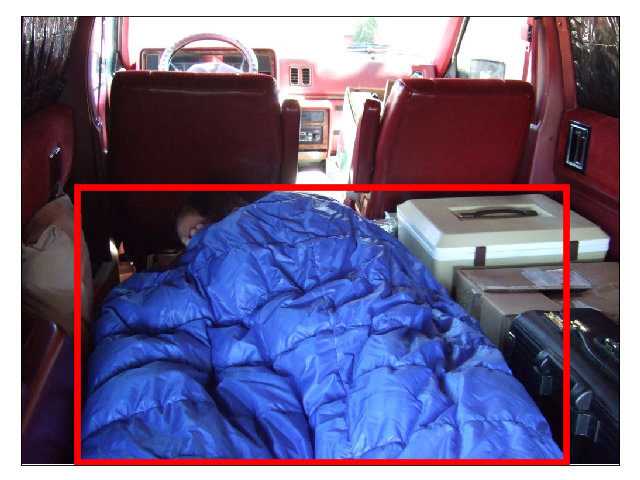
\includegraphics[width=0.9\linewidth]{figures/498222_3135415_singleton_obj.png}} bed (12), sleeping bag (9), blanket (7), bed sheet (5)\\ 
\multicolumn{4}{c}{\textbf{VG: batter}}\\
\raisebox{-\totalheight}{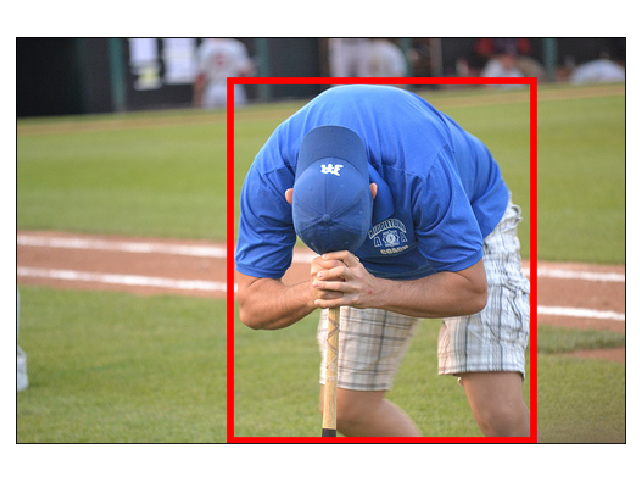
\includegraphics[width=0.9\linewidth]{figures/2372219_2683892_supercat_unique.png}} man (24), cap (5), person (3), baseball player (2) &
  \raisebox{-\totalheight}{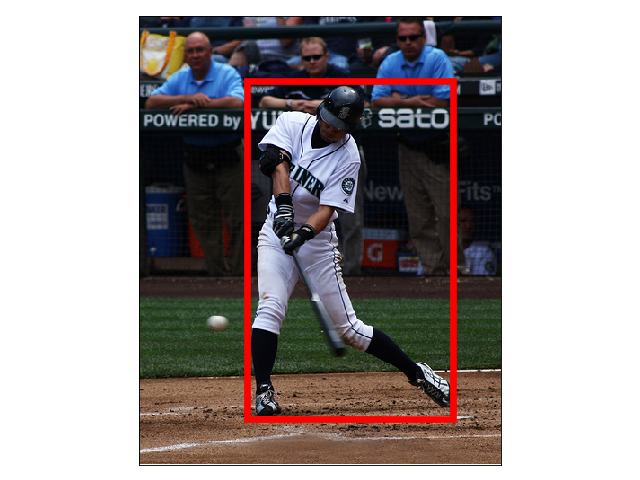
\includegraphics[width=0.9\linewidth]{figures/2394377_464684_singleton_obj.png}} man (13), baseball player (7), batter (5), player (3), helmet (2) &
\raisebox{-\totalheight}{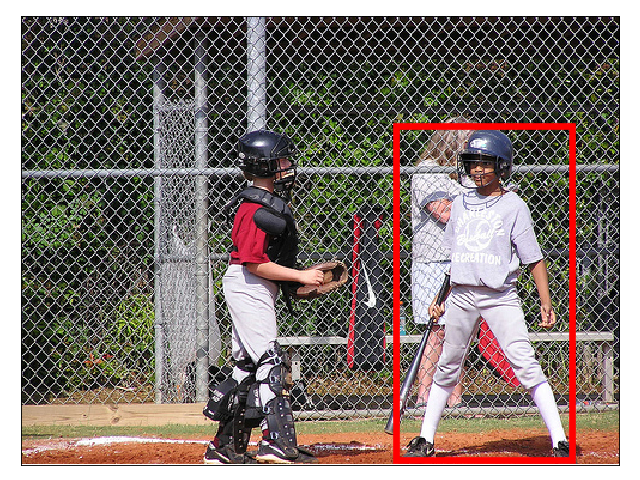
\includegraphics[width=0.9\linewidth]{figures/2398907_2901496_singleton_obj.png}}  boy (7), helmet (5), baseball player (4), player (4), man (3), child (3), batter (3), dress (2), kid (2)&
\raisebox{-\totalheight}{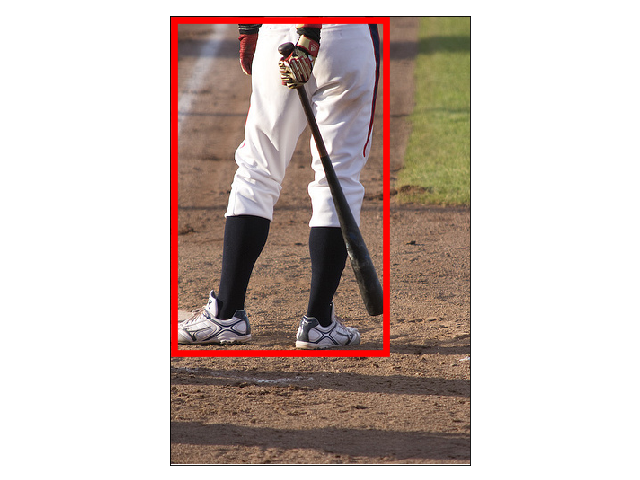
\includegraphics[width=0.9\linewidth]{figures/2337552_957263_singleton_obj.png}} pants (6), player (5), shoe (4), bat (4), person (4), legs (4), baseball player (3), hitter (2)\\ 
\multicolumn{4}{c}{\textbf{VG: robe}}\\
\raisebox{-\totalheight}{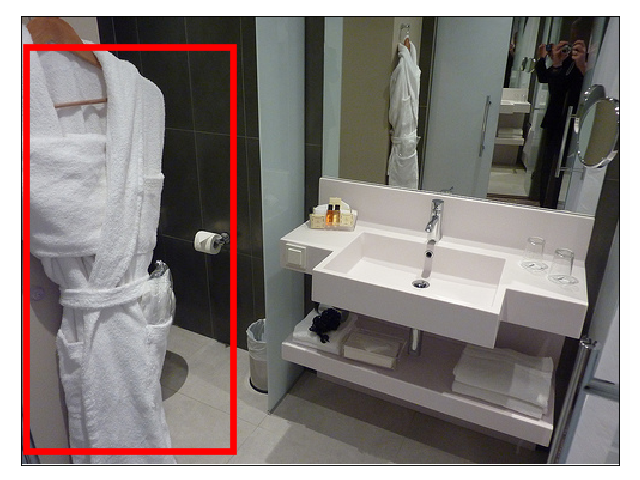
\includegraphics[width=0.9\linewidth]{figures/2373180_2333161_singleton_obj.png}} robe (27), bathrobe (5) &
  \raisebox{-\totalheight}{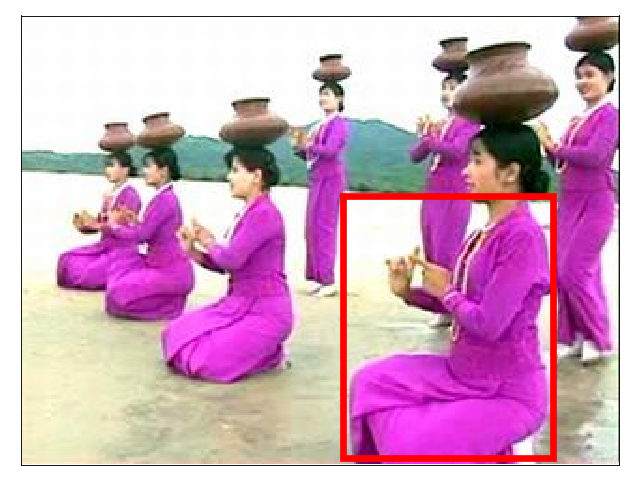
\includegraphics[width=0.9\linewidth]{figures/160_1058761_supercat_unique.png}} dress (30), uniform (2) &
\raisebox{-\totalheight}{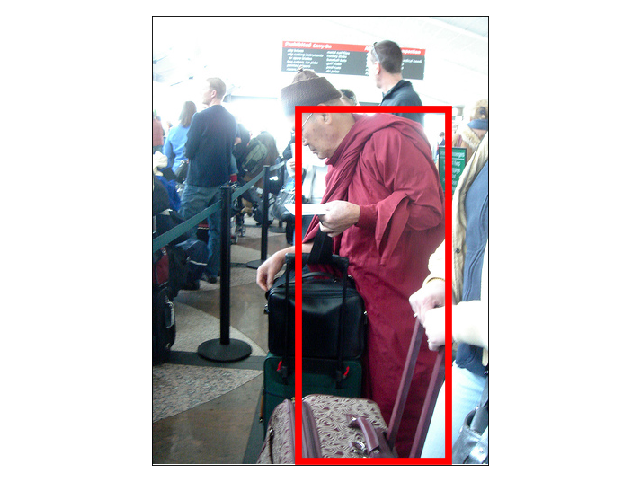
\includegraphics[width=0.9\linewidth]{figures/2334612_2838713_supercat_unique.png}}  robe (11), jacket (7), clothes (6), bag (3), dress (2), man (2) &
\raisebox{-\totalheight}{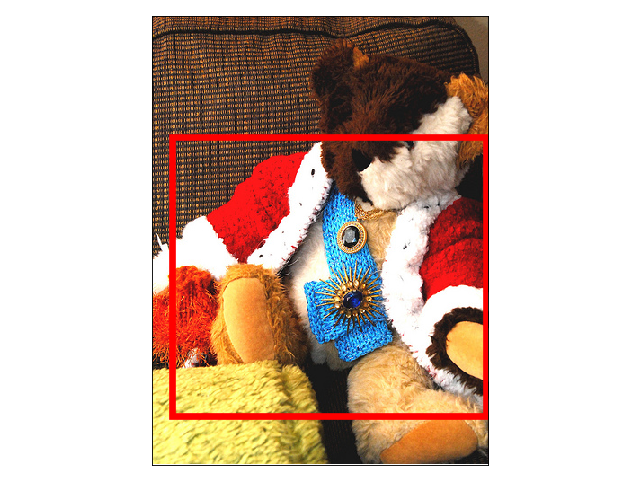
\includegraphics[width=0.9\linewidth]{figures/2340041_2137546_supercat_ambiguous.png}} jacket (10), sweater (9), coat (3), doll (3), toy (3), shirt (2), bear (2), robe (2)\\ 


\end{tabular}

}
\end{minipage}

 \caption{\label{fig:ex}Examples for different instances of VG synsets with low and high agreement in MN data set}
\end{figure*}



%\gbt{The non-canon. VG names suggest that people prefer more general names (``car $>$ sedan'', ``horse $>$ pony'', ``tie $>$ necktie''). Could be due to lexical availability (more general \ra more frequent \ra more available). This could be verified (using frequency). Hypothesis: In cases where top name != VG, the VG name is less general. Could be also a more general hypothesis: see if people prefer more frequent names in general.}
%\cs{@Table~\ref{tab:qual} (just wrt presentation) The most interesting blocks are 2 and 3 (canonical VG with min agr.; non-canonical with max agr.)}


\subsection{Discussion (for now)}
What does this discrepancy between the instance-level and category-level agreement in VisualGenome and ManyNames naming choices mean? 
First of all, it suggests that the same original VisualGenome name can trigger very different variants depending on the visual instance, leading to a drastic increase of variants elicited for categories as compared to instances.
Second, this clearly shows that annotators in VG do not generally annotate the most canonical name \cs{but they don't annotate the name, but the description} and that many names annotated for objects in VG do not correspond to the overall most preferred variant. \sz{think more ...}
\gbt{I don't think we can conclude this second part -- we do have the 70\% top=VG figure that says that VG annotators annotate the most canonical name. What this suggests to me is that instance-level properties are more important than category-level properties, somehow.
  That is, there are systematic properties of instances that make them have a single most salient name.
  However, I expect that this result will be very influenced by referential uncertainty (in single images, it will mostly be clear that it's a man, but in some it may be unclear \ra high instance agreement, low category agrement.}
\cs{I don't think that 70\% is high. E.g., the ResNet has a top-1 error rate of 25\% on ILSVRC 2015.}

\cs{(?!?) With respect to implications for L+V  models on language *interpretation*: much lower agreement on object class-level than on instance-level speaks for using very fine-grained object annotations (as done in ILSVRC). 
	However, that naming variants are often not explained/recoverable by hierarchical relations questions in how far models can understand/interpret reference to objects using more general classes (i.e., names), despite being able to recognise an object's very specific class (e.g., ILSVRC synset). (Relevant?!?)}

\begin{table*}
\footnotesize
%\begin{tabular}{p{1.3cm}cccccc|cccccc}
%\toprule
% & \multicolumn{6}{c|}{Instance-level agreement} & \multicolumn{6}{c}{Class-level agreement}\\ 
%           domain & \% top &    $H$ &    N & N$_{>1}$ & top=VG &  \% VG & \% top &    $H$ &     N & N$_{>1}$ & top=VG &  \% VG \\
%\midrule
%            all &  69.7 (22.2) &  1.3 &  5.7 &   2.9 &  72.8  &  58.7  &   52.6 (21.1) &  2.4 &   62.2 &  29.7 &  32.7 (46.9) &  23.5 (27.0)  \\
% \midrule
%         people &  51.9 (18.1) &  2.1 &  8.6 &   4.3 &         49.8 &         32.3 &     43.1 (14.9) &  2.9 &  104.4 &  53.4 &         24.4 &         13.2  \\
% animals\_plants &  91.3 (12.9) &  0.4 &  2.7 &   1.5 &         93.8 &         88.0 &     67.9 (23.5) &  1.5 &   26.7 &  12.4 &         29.5 &         26.2  \\
%       clothing &  63.9 (17.9) &  1.6 &  6.4 &   3.2 &         70.2 &         52.6 &     49.3 (16.6) &  2.6 &   71.7 &  34.1 &         40.5 &         26.1  \\
%       vehicles &  72.0 (19.5) &  1.1 &  4.7 &   2.4 &         71.1 &         60.2 &    54.4 (17.4) &  2.1 &   70.4 &  33.2 &         21.4 &         21.3  \\
%      buildings &  66.9 (20.5) &  1.5 &  6.9 &   3.0 &         72.6 &         55.5 &      46.7 (18.2) &  3.0 &   68.5 &  31.3 &         32.3 &         22.3  \\
%           home &  66.4 (20.5) &  1.5 &  6.3 &   3.1 &         78.5 &         58.8 &     49.6 (18.7) &  2.8 &  103.2 &  48.8 &         45.9 &         30.1  \\
%           food &  71.3 (21.1) &  1.3 &  5.5 &   2.9 &         62.9 &         52.1 &     47.3 (19.5) &  2.5 &   32.1 &  15.2 &         31.1 &         20.8  \\
%\bottomrule
%\end{tabular}

\begin{tabular}{lccccc|ccccc}
\toprule
 & \multicolumn{5}{c|}{Instance-level agreement} & \multicolumn{5}{c}{Class-level agreement}\\ 
          domain &    N &         \%top (std) &          H (std) & top=VG &   \%VG &     N &         \%top (std) &          H (std) & top=VG &   \%VG \\
\midrule
            all &  2.9 &  75.2 (21.9) &  0.9 (0.7) &   72.8 &  62.8 &  29.7 &  56.4 (21.5) &  2.0 (1.0) &   32.7 &  23.4 \\
       vehicles &  2.4 &  76.6 (19.8) &  0.8 (0.6) &   71.1 &  63.9 &  33.2 &  57.4 (17.3) &  1.8 (0.6) &   21.4 &  21.2 \\
      buildings &  3.0 &  74.7 (20.7) &  1.0 (0.7) &   72.6 &  61.6 &  31.3 &  51.0 (18.8) &  2.4 (0.9) &   32.3 &  22.2 \\
       clothing &  3.2 &  70.1 (18.5) &  1.1 (0.6) &   70.2 &  57.4 &  34.1 &  53.4 (16.6) &  2.1 (0.8) &   40.5 &  26.1 \\
           home &  3.1 &  72.6 (20.7) &  1.0 (0.7) &   78.5 &  64.1 &  48.8 &  54.0 (19.4) &  2.3 (1.0) &   45.9 &  29.9 \\
         people &  4.3 &  59.0 (20.4) &  1.5 (0.7) &   49.8 &  36.3 &  53.4 &  47.5 (17.2) &  2.5 (0.9) &   24.4 &  13.0 \\
           food &  2.9 &  76.4 (20.7) &  0.9 (0.7) &   62.9 &  55.2 &  15.2 &  50.8 (20.3) &  2.0 (0.8) &   31.1 &  20.8 \\
 animals\_plants &  1.5 &  94.5 (12.1) &  0.2 (0.4) &   93.8 &  91.0 &  12.4 &  71.3 (23.3) &  1.2 (0.9) &   29.5 &  26.1 \\
\bottomrule
\end{tabular}

\caption{Agreement in naming measured on the level of instances and on the level of VG classes (i.e.\ after grouping objects by their VG synset), for filtered response sets (frequency threshold of 2)}
\label{tab:agree}
\end{table*}


%Why is naming more flexible in certain domains than in others? \gbt{Hypothesis: expectation: little variation - hypernymy at most, more variation <-> more affordances <-> more varied relationships.}



\cs{@Table~\ref{tab:agree} I still think that we could also have \%\ top with $N>1$ to give an idea as to how useful the data is for the people interested in using it for, e.g., model evaluation. For that, it is clear that crowdsourcing is noisy and before using it some outlier removal needs to be made.}

% \subsection{Entry-level names and preference orders....}

% \sz{an interesting example:} In our data set, there are 24 images where \textit{penguin} has been used, so we know that the object is a \textit{penguin}. For 50\% of these images, annotators still prefer \textit{bird} as the most common name. According to the theory of entry-level categories, this should not happen. People should always prefer \textit{penguin} over \textit{bird}. 

% \sz{how can we analyze this quantitatively?}

% \begin{itemize}
% \item lettuce -- salad
% \item fruit -- food
% \item man -- catcher
% \item bowl --chili
% \item bowl -- diner \gbt{spelling mistake? should be dinner?} 
% \item burger -- meat
% \item statue -- animal (image shows statue of an animal)
% \item bottle -- alcohol
% \item donut --desert \gbt{spelling mistake? should be dessert?} 
% \item zebra -- stripes
% \item oven -- grill
% \end{itemize}


%%% Local Variables:
%%% mode: latex
%%% TeX-master: "main"
%%% End:


\section{Conclusion}
\label{sec:conc}
% To sum up, we find both substantial consistency in naming (the most frequent name accounts for 75\% of object names, on average) and substantial naming variation (the remaining 25\%). Moreover, there is a very large standard variation in how much agreement there is for objects in images, that only partially depend on the domain.

The question of how people choose names for objects presented visually is relevant for Language and Vision, Computational Linguistics, Computer Vision, Cognitive Science, and Linguistics.
We have surveyed datasets that can be useful to address this question, and proposed a new dataset, ManyNames, that affords new possibilities both for analysis and modeling of object naming.
% gbt: commenting the following out cause it's a bit dangerous to say this without the verification phase.
% , providing a means
% (i) to study how different people would name the same object (image region), and, given a specific name, estimate how likely people are to use it for a given object, which might vary substantially across different instances of a given category, and
% (ii) to obtain a set of possible names for individual objects, as well as available lexical alternatives for specific names, which again might vary strongly across instances and often cannot be retrieved from existing taxonomies like WordNet. 

For Computer Vision and L\&V, our data highlights the fact that bounding boxes are often ambiguous, which can affect model performance on object categorization and naming.
Crucially, evaluations in these tasks assume that object identification is possible based on the bounding box; beyond showing that this is not always the case, our data can be used to assess whether model mistakes are plausible (similar to those of humans, as in the \word{toy/book/bed} case), or really off.

Moreover, standard evaluations assume that object names (or categories) are unique.
% The naming variation we have found also challenge the common assumption that there exists a single canonical name for individual visual objects (also see \cite{deng2014large,wang2014poodle,peterson2018learning}).
The ability to distinguish incorrect object names from good alternatives is essential for visual object understanding.
Our data provides a first step towards enabling model evaluation on naming variants of an instance, checking, e.g.,\ to what extent the top N predicted names are valid alternatives (\word{dog, animal, pet}) or not (\word{dog, hat, grass}).
However, to fully enable this sort of analysis, a further annotation step is needed, to account for the referential uncertainty of bounding boxes and annotation noise.
We plan to take this step in future work, which will also enable more robust conclusions with respect to naming variation.

% Wang et al.: ". The hypothesis is that by modeling the variation in granularity levels for different concepts, we can gain a more informative insight as to how the output of image annotation systems can relate to how a person describes what he or she perceives in an image, and consequently produce image annotation systems that are more human-centric."
% @related work
%[For example, \newcite{peterson2018learning} train CNN classifiers on objects with multiple labels which stand in a hierarchical relation (e.g., dog, animal) in order to learn better visual representations which capture the hierarchical structure of a taxonomy. \cs{remove or move to related work? also sentence to Ordonez}]
%\footnote{Other work used training data with multiple labels per image to improve image classification performance on images with multiple objects (e.g.,~Wang et al., 2016 REF). \cs{maybe remove, since it is not that relevant?}}
% peterson2018learning: discuss the bias introduced into learned representations by training on data of  single label annotations ("labels cut arbitrarily across natural psychological taxonomies, e.g., dogs are separated into breeds but never categorized as dogs"). 

% However, given the fact that naming variants are often not recoverable by hierarchical relations, a taxonomic hierarchy is only limited in its use to distinguish automatically a truly false prediction (e.g.,\ \textsl{plate}) from a (possibly context-specific) valid alternative (e.g.,\ \textsl{basket}) to the single "ground truth" in a dataset (e.g.,\ \textsl{sandwich}). 
% For the same reason, even fine-grained recognition models (as those trained on ILSVRC) cannot be expected to be able to simply infer the recognition of more general classes.
%since we found that many name alternatives are not hierarchically related to the VG name, there is only limited use of, e.g., a taxonomic hierarchy, to distinguish automatically a "truly" false prediction (e.g.,\ \textsl{plate}) from a (possibly context-specific) valid alternative (e.g.,\ \textsl{basket}) to the single "ground truth" in a dataset (e.g.,\ \textsl{sandwich}). 

With respect to naming variation, our current data supports the prediction in theoretical research on object naming that there will often be a preferred (entry-level) name for a given visually presented object.
It tentatively suggests that (a) there is also consistent variation in naming, with an average of almost three elicited names per instance; (b) much of this variation cannot be explained by adopting a hierarchical view, which has been dominant in the psycholinguistic and computational literature; (c) there is high variability in agreement across instances within the same domain.
The latter suggests that there are specific visual characteristics of either the object itself or the visual context in which it appears that trigger variation. With prototypical, idealized pictures of the sort used in traditional studies (see Figure\ \ref{fig:cake}), this observation would not be possible.

We hope that ManyNames triggers more empirical research on object naming, a topic that has been understudied in both computational and theoretical approaches to language.

%%% Local Variables:
%%% mode: latex
%%% TeX-master: "lrec2020naming"
%%% End:


 \section{Acknowledgements}

% Place all acknowledgements (including those concerning research grants and
% funding) in a separate section at the end of the article.

\section{Bibliographical References}
\label{main:ref}

\bibliographystyle{lrec}
\bibliography{naming}


%\section{Language Resource References}
%\label{lr:ref}
%\bibliographystylelanguageresource{lrec}
%\bibliographylanguageresource{lrec2020W-xample}

\end{document}

%%% Local Variables:
%%% mode: latex
%%% TeX-master: t
%%% End:
